\chapter{FOSS projects as Cohesive Small Worlds}
\label{cohesive_small_world}

As discussed in chapter \ref{collaborative_communities}, we named ``collaborative small world'' the network model that we propose in order to theoretically understand the structural dimension oc cooperation of FOSS projects. We argued that the family of networks that fit in the intersection of small world networks and structural cohesion networks exhibit consistent topological patterns. These patterns, we argue, provide the scaffolding for the emergence of collaborative communities. On the one hand, the generation of trust and congruent values among heterogeneous individuals are fostered by structurally cohesive groups in the network that play a key role in amplifying the effects of social interactions trough relatively long paths. On the other hand, the existence of highly connected local clusters linked together by relativelly small paths ---compared to suitable random networks--- allows successful collaboration among heterogeneous individuals with common interests even though they geographically dispersed and might never meet face to face.

This chapter focus on the empirical analysis of the network structure of two mature and well stablished FOSS projects: the CPython reference implementation of the Python programming language and the Debian Operating System. These two projects, as outlined in the previous chapter, are quite different despite being both successful FOSS projects. The Debian project has approximately ten times more participants than Python. Debian, being a complete Operating system, has many parts which are only lightly related between them becuse it contains programs that do very different tasks (eg the developers working on packaging software for music editing do not need to pay close attention to what devian developers focused on packaging word processors do). On the other hand, the Python programming language is a much more integrated software projects, and thus developers working on different parts of the language implementation have to play attention, and work very closely, with other developers.

This has a strong impact in the structure of the patterns of relations that emerge between developers in the two projects. The analysis presented here has two parts: first we will compute the small world metrics for the two projects, as described in chapter \ref{collaborative_communities}, and then we will compute the structural cohesion metrics as described in the chapter \ref{structural_cohesion}. However first we have to define how we build the networks for this two projects as a formalizations of the patterns of cooperation between the individuals in these projects.

\section{Modeling patterns of cooperation as networks}

Our modeling strategy to capture the patterns of relations among developers in these two projects is to focus on the actual contributions of each developer to the project. We model the cooperation patterns between individuals as affiliation networks \citep[chapter 8]{wasserman:1994}. This kind of networks contain two types of nodes: $N$ actors each of which belongs to one or more groups $M$. Such networks are bipartite or 2-mode because they contain two types of nodes and there are no edges between nodes of same type.

The two sets of nodes in the networks analyzed here are, on the one hand, human developers and, on the other hand, entities that conform the product that is released by the FOSS project. In the case of Debian, these entities are software packages, and in the case of Python, they are source code files. Note that the collaboration network is based on individual contribution but it not only captures the total amount of contribution that a given individual does, but also to which part of the project the contributions are focused, and who else in the project is also working on the same entities. This is why we name these bipartite graphs collaboration or cooperation networks.

One feature of most large software projects is modularity, that could be defined as the division of a software project into semi-independent parts, designed to work together but that can be developed relatively independently. In the case of an operating system, such as the Debian project, modularity is more important than in other software projects, such as Python. An operating system comprises a comprehensive set of software packages with varying importance, from those responsible for interacting with the hardware to others that provide certain features that are only useful in very specific and specialized configurations. On the other hand, an implementation of a programming language, such as Python, is also modular but their parts are much more closely related and have to be tightly integrated in order to function as a coherent whole.

This modeling approach captures mostly the informal patterns of relations that individuals establish when contributing to the project. FOSS projects have a wide range of formal organizational forms, and in this respect, they can be quite different. The definition of the leadership position in the two projects in which we focus this thesis nicely capture these differences in formal organization: Debian has a very developed formal bureaucracy, the project elects its leader each year through a secret vote of all its members after a electoral campaign where the candidates discuss among them and try to gain supports; Python instead has its original author ---Guido van Rossum--- in a permanent position of leadership, the people in the project refer to him, and his position of leadership, as ``Benevolent Dictator For Life'' (BDFL).

Despite these differences in the formal organization, if we focus on the patterns of relations among developers in the productive process, what we call the cooperation network, we can analyze the contribution dynamics, analyze hierarchical positions defined by these patterns, assess the pace of renewal in these positions, and determine the impact in the median active life on a developer in a project of being in a concrete hierarchical position.

For the case of the Debian project, we define that each package of source code is a module of the system or, in terms of network affiliation, a group or team. The main data source is the Ultimate Debian Database (UDD)\footnote{\href{http://udd.debian.org/}{http://udd.debian.org/} [accessed November 2016]} \citep{udd:2010}. The UDD contains information related to the work of each individual in the project which allow us to build the developers-packages affiliation network. One developer is linked to every package she has uploaded in the archive in a period of one year. Therefore, the result is a 2-mode network with developers ---the actors--- and packages ---the groups--- as the two types of nodes.

For the case of the Python project, we define that each source code file that forms the reference implementation of the programming language is a module of the system or, in terms of network affiliation, a group or team. Thus, contributions are lines of source code added or deleted from one of the source code files of Python's code base. The main data source is the Python source code repository \footnote{\href{https://hg.python.org/cpython}{https://hg.python.org/cpython} [accessed November 2016]}, which is under version control. That means that each change to any source code file is recorded and attributed to a person.

These collaboration relations are only part of the whole patterns of cooperative relations established among developers in both projects. We cannot obtain more accurate data of the frequent interactions between developers related to the production process that take place in a large variety of on-line or face-to-face settings. However, the subset of collaboration relations captured by our approach are significative and serve our purpose to analyze the global patterns of relations among direct producers because the result of the productive process is, in fact, the archive of packages that form the Debian operating system or the set of source code files taht form the implementation of the Python programming language. Therefore, we base our analysis of cooperation on the registered contribution of each developer to the final product of the productive process delivered to end users.

Moreover, two important advantages of this approach are, on the one hand, that we have data on all uploads ---in the case of Debian--- or all the modifications of source code files ---for the Python project---, thus we do not need to worry about sample bias because we have accurate data of all the work performed in the period under analysis. On the other hand, we have a strict definition of what cooperation means, which allow us analyze the evolution of collaboration patterns throughout the history of the two projects. Therefore, we can make meaningful comparisons between years in the same project, and between projects.

\subsection{Null models}

Both kinds of analysis presented in this chapter have in common the use of null models. In empirical analysis of networks we need to be able to compare the statistical measures obtained of our actual networks with a null model in order to assert that what we observe is not the result of pure chance. That is, we have to make sure that the metrics observed in the actual networks are significantly different to the patterns of relations that we might expect if the relation between developers and packages, or developers and files in the case of Python, were produced uniformly at random.

To this end, the canonical approach is to compare the measures of actual networks with measures taken from random networks that maintain some constraints of the original network, such as the degree distribution. \citet*{newman:2003,nsw:2001} provided a configuration model in order to generate random graphs with arbitrary degree distributions. In the analysis presented here we have used the configuration model for 2-mode networks to generate 100 random null models for each year. The configuration model assigns at random developers to packages, or developers to source code files, maintaining the concrete skewed distribution of packages by developer and files by developer observed in the actual networks.

In order to compute the small world metrics reported in the next section, I've used the mean of the relevant statistics from ten random networks selected uniformly at random from a pool of one hundred random networks ---generated using the configuration models described above. I did some test increasing one order of magnitude these figures ---that is, selecting one hundred random networks from a pool of one thousand--- and the results were the same up to the second decimal of the relevant statistics.

For the case of structural cohesion null models, it's not possible to use the mean because what we have to compute is the whole connectivity structure, and it's graphical representation requires to use only one network. Thus I've used only one random configuration model network as a null model for the structural cohesion analysis.  

\section{Small World Metrics}

As we discussed in chapter \ref{collaborative_communities}, a network fits the small world model if it is more clustered ($CC$) than its random network counterpart but has approximately the same average distance ($L$) between nodes. In unipartite or 1-mode networks, $CC$ is the mean probability that two nodes that are neighbors of the same other node will themselves be neighbors. Thus, this measure is computed as the ratio of triangles ---a fully connected graph of 3 nodes--- over two-stars ---three nodes connected by two edges---. But, in bipartite or 2-mode networks there can be no triangles because, by definition, edges can only link nodes of different type. Following \citet{robins:2004}, \citet{lind:2005} and \citet{latapy:2008}, local cohesion in 2-mode networks can be measured with the notion of cluster coefficient based on squares ($CC_4$). $CC_4$ is the ratio between the number of squares ($C_4$) ---composed by two nodes of each type linked by four edges--- over the number of three-paths ($L_3$) ---composed by two nodes of each type linked by three edges--- (See appendix \ref{sw-affnets} for a formal definition of $CC_4$). Like $CC$, $CC_4$ applied to bipartite networks is a measurement of local cohesion.

The Small World Index ($Q$) is a summary indicator of the smallworldiness of a network and accounts for both the relation of the clustering coefficients of actual networks compared to their random counterparts, and the relation of average path length (a global measure of the average distance between nodes in a network) of actual networks compared to their random counterparts. Networks with the Small World Index ($Q$) bigger than 1 are considered small world networks (see appendix \ref{sw-affnets} for details). We compute the Small World Index using the following formulas:

\begin{equation}
% \begin{split}
Q = \frac{CC_{ratio}}{L_{ratio}}
% \end{split}
\end{equation}

Where:

\begin{align}
CC_{ratio}& = \frac{CC_{actual}}{CC_{random}} &
L_{ratio}& = \frac{L_{actual}}{L_{random}} \nonumber \\
\end{align}

In the tables below, $CC_{actual}$ is column column 6, $CC_{random}$ is column 7, $L_{actual}$ or average path length (APL) is column 8, $L_{random}$ is column 9, and the Small World Index $Q$ is column 10.

In the first place we compute small world metrics for Debian networks. The results are shown in table \ref{swi_debian}.

\begin{table}
\begin{center}
\begin{tabular}{|c|c|c|c|c|c|c|c|c|c|}
\hline
Years&Nodes&Developers&Packages&Edges&CC&random CC&APL&random APL&SWI ($Q$)\\
\hline
1999&3258&391&2867&3250&0.127&0.002&9.4&8.8&54.4\\
2000&3590&521&3069&3493&0.136&0.002&9.5&8.9&80.4\\
2001&5921&755&5166&6158&0.050&0.001&8.4&7.9&31.9\\
2002&6839&840&5999&7109&0.079&0.001&9.2&8.0&48.3\\
2003&7244&882&6362&7764&0.102&0.002&9.0&7.7&56.9\\
2004&7971&982&6989&9390&0.155&0.002&8.0&6.6&52.3\\
2005&8317&1037&7280&10242&0.169&0.003&7.5&6.2&44.1\\
2006&9564&1127&8437&12863&0.173&0.005&6.7&5.6&31.7\\
2007&9434&1145&8289&12736&0.144&0.004&6.8&5.6&26.7\\
2008&10605&1212&9393&14226&0.188&0.004&7.1&5.6&33.1\\
2009&11284&1293&9991&15538&0.229&0.006&7.0&5.4&30.8\\
2010&10447&1319&9128&13702&0.282&0.005&7.7&5.6&40.2\\
2011&12265&1333&10932&15862&0.141&0.005&7.5&5.5&21.3\\
2012&8408&1055&7353&9528&0.162&0.003&9.5&6.2&32.9\\
\hline
\end{tabular}
\caption{Small world metrics for debian networks.}
\label{swi_debian}
\end{center}
\end{table}



As we can see, the Debian project cooperation networks for all years analyzed are indeed small world networks. Their Small World Index ($Q$) is quite bigger than 1, ranging from 21.4 in 2011 to 97 in year 2000. This large value of $Q$ is driven by the fact that the clustering coefficient ---the measure of local cohesion--- of the observed networks is approximately a hundred times higher than in their random counterparts. However the average distance between nodes in the actual networks is slightly higher than the distance in their random counterparts, which reduces the value of the small world index. Therefore we can conclude that Debian cooperation networks fit nicely the small world model. 

Note that the Small World Index ($Q$) is quite stable compared with the huge increment of the number of developers involved in the Debian project and the number of software packages uploaded to the Debian repository. The number of developers grows quickly the first years under analysis, but tends to stabilize in the 2010s. There where 392 active developers in 1999 who uploaded 2,867 software packages that year; in 2012 there were 1,435 active developers who uploaded 10,469 packages. That is a bit more than a three fold increment.

The high value of the Small World Index in the Debian project compared to its value in the Python project ---which we discuss below--- is because Debian as an Operating System is more modular than Python as a programming language. Thus it's much more common in Debian to have subgroups of developers that work only in a small set of packages independently of other subgropus of developers.

For the Python project, the results for the small world metrics are presented in table \ref{swi_python}.

\begin{table}[H]
\begin{center}
\begin{small}
\begin{tabular}{|c|c|c|c|c|c|c|c|c|c|}
\hline
Years&Nodes&Developers&Files&Edges&CC&random CC&APL&random APL&SWI ($Q$)\\
\hline
1999&1,146&9&1,137&1,236&0.102&0.039&3.1&3.5&3.0\\
2000&2,172&31&2,141&3,720&0.214&0.135&3.3&3.5&1.7\\
2001&2,511&33&2,478&4,507&0.205&0.129&3.4&3.6&1.7\\
2002&2,317&38&2,279&4,502&0.204&0.129&3.6&3.6&1.6\\
2003&1,805&42&1,763&3,192&0.153&0.112&3.5&3.6&1.4\\
2004&1,850&49&1,801&3,163&0.113&0.093&3.4&3.6&1.3\\
2005&1,007&44&963&1,759&0.129&0.079&3.7&3.7&1.7\\
2006&2,632&52&2,580&6,794&0.235&0.156&2.8&3.2&1.7\\
2007&3,359&51&3,308&7,790&0.223&0.177&2.9&3.3&1.4\\
2008&2,951&59&2,892&7,833&0.231&0.175&3.0&3.3&1.5\\
2009&2,219&58&2,161&4,708&0.228&0.142&3.1&3.4&1.7\\
2010&2,930&63&2,867&6,504&0.175&0.128&3.4&3.5&1.4\\
2011&2,174&63&2,111&4,459&0.145&0.114&3.5&3.6&1.3\\
2012&2,444&65&2,379&4,843&0.124&0.087&3.7&3.8&1.4\\
2013&2,285&63&2,222&4,743&0.147&0.099&3.6&3.7&1.5\\
2014&2,134&62&2,072&4,149&0.138&0.095&3.6&3.7&1.5\\
\hline
\end{tabular}
\caption{Small world metrics for python networks.}
\label{swi_python}
\end{small}
\end{center}
\end{table}



In the case of the Python project, the Small World Index ($Q$) is still greater than one in all years analyzed, ranging from 3 in 1999 to 1.3 in 2004 and 2011. The value of $Q$ in this case is driven by the small average distance between nodes in the cooperation networks. Most years Python networks have an average path length $L$ slightly smaller than their random networks counterparts, while their clustering coefficient $CC$ is bigger than their null models, but not by much. We can still confidently conclude that the Python project cooperation networks also fit the small world model.

In this case, the Small World Index ($Q$) is remarkably stable during all years under analysis. In 1999, when only 9 developers edited 1,137 source code files, the value of $Q$ was 3. The following years its walue stabilized arround 1.5 despite the fact that the number of developers participating activelly in the project increased steadily until reaching approximately 60 developers in 2010, and maintaining this number from 2010 to 2014. Thus on the period analyzed the developers activelly editing source code files in the project multiplied by seven.

The low value of the Small World Index ($Q$) in the Python project, compared with the values of $Q$ in the Debian project, can be attributed to the lower modularity of Python as a programming language compared with the inherent modularity of the Debian project as an operating system. The need of tight integration between parts of the same programming language make more difficult for subgroups of developers to work independently in subsets of source code files independently of other developers. 

\section{Structural Cohesion Analysis}

As discussed in chapter \ref{structural_cohesion} our approach to the analysis of structural cohesion of cooperation networks is based on the work of \citet{white:2001} and \citet{moody:2003}. The cohesive structure of a network can be conceptualized as increasingly cohesive groups nested inside each other. A common structural pattern in large networks is an hierarchical nesting of increasingly cohesive groups at low connectivity levels and non-overlapping highly cohesive groups at higher connectivity levels \citep[112]{moody:2003}. Those highly cohesive groups play a key role in the diffusion of the consequences of social interactions among actors in networks \citep[355-356]{white:2001}. It is usually assumed that the transmission through the network of knowledge, influence and resources generated by social interactions is limited to people 2 or 3 steps away from the initiator of such interactions. In graph theoretic terms, this means that social interactions have a high rate of decay. However, strongly cohesive blocks allow repetition of information and reinforcement of influence because they are characterized by multiple independent pathways that compensate the decay effects of the transmission of knowledge, influence and resources.

This key feature of cohesive groups provides a plausible social mechanism for the emergence and development of trust in collaborative communities. Actors in strongly cohesive groups are able to compare independent perspectives on each other through a variety of paths that flow through distinct sets of intermediaries, which provides multiple independent sources of information about other's characteristics or identity \citep[320]{white:2001}. Thus, the perception of an individual embedded in such structures of the other members of the group to whom he is not directly linked is filtered by a the perception of a variety of others whom he trusts because is directly linked to them. This mediated perception of the group generates trust at a global scale, which according to \citet{adler:2006} is the key mechanism for the development of collaborative communities, as discussed in chapter \ref{collaborative_communities}.

The analysis presented in this section are only possible thanks to the heuristics that we developed in order to be able to deal with networks of tens of thousands of nodes and edges as described at length in chapter \ref{structural_cohesion} and appendix \ref{appendix_cohesive_groups}. 

Table \ref{str_cohesion_python} presents the first step of the analysis for the Python cooperation networks.

\begin{table}[H]
\begin{center}
\begin{tabular}{|c|c|c|c|c|c|c|c|}
\hline
Years&Nodes&GC&Random GC&GBC&Random GBC&maximum $k$&Random max $k$\\
\hline
1999&1146&66.0\%&100.0\%&6.7\%&6.5\%&3 (1.0\%)&2 (6.5\%)\\
2000&2172&96.5\%&100.0\%&33.4\%&31.4\%&8 (1.2\%)&5 (3.1\%)\\
2001&2511&97.3\%&99.8\%&34.1\%&33.0\%&9 (1.2\%)&6 (2.4\%)\\
2002&2317&100.0\%&99.8\%&38.1\%&36.9\%&9 (2.6\%)&7 (1.9\%)\\
2003&1805&100.0\%&99.2\%&34.8\%&33.1\%&7 (3.3\%)&6 (2.4\%)\\
2004&1850&99.8\%&100.0\%&39.7\%&37.1\%&7 (1.8\%)&5 (2.5\%)\\
2005&1007&99.8\%&100.0\%&45.7\%&44.2\%&5 (5.8\%)&4 (7.6\%)\\
2006&2632&100.0\%&100.0\%&74.2\%&69.8\%&9 (1.5\%)&6 (3.9\%)\\
2007&3359&100.0\%&100.0\%&58.6\%&55.2\%&9 (2.0\%)&6 (2.2\%)\\
2008&2951&100.0\%&99.9\%&64.5\%&61.7\%&10 (2.2\%)&7 (2.5\%)\\
2009&2219&100.0\%&99.9\%&51.0\%&48.5\%&7 (2.8\%)&5 (5.6\%)\\
2010&2930&100.0\%&99.9\%&48.7\%&47.0\%&9 (2.7\%)&7 (2.4\%)\\
2011&2174&100.0\%&99.8\%&47.7\%&45.9\%&8 (2.9\%)&7 (1.7\%)\\
2012&2444&99.8\%&99.8\%&41.1\%&40.3\%&8 (3.4\%)&7 (3.4\%)\\
2013&2285&99.9\%&99.9\%&51.6\%&49.8\%&7 (4.2\%)&6 (4.0\%)\\
2014&2134&100.0\%&99.8\%&44.6\%&43.4\%&7 (2.6\%)&6 (3.1\%)\\
\hline
\end{tabular}
\caption{Structural Cohesion metrics for python networks.}
\label{str_cohesion_python}
\end{center}
\end{table}



This table contains the total number of nodes of the cooperation network for each year analyzed on the column named ``Nodes''. The column labeled ``GC'' contains the percentatge of the total nodes that are part of the giant component of the cooperation network, and the column labeled ``GC random'' is this same percentage but for a random configuration model network which we use as a null model. This metric is important because the starting point of the social cohesion in a network is a state where every actor can reach every other actor through at least one relational path. The formalization of this state in a concrete network is the size of the largest connected component which is what these columns report. 

The column labeled ``GBC'' contains the percentage of nodes that are part of the giant bicomponent of the cooperation network, and the column labeled ``GBC random'' is the same percentage for their random network counterpart. \citet{moody:2003} argue that the removal of a few key nodes can affect the flow of knowledge, information and resources in a connected component because it only has at least one relational path between any two nodes. In network terms, a graph is $k$-connected and is called a $k$-component if you need to remove at least $k$ nodes to break it into more components. A 2-component, or bicomponent is a component that requires at least 2 nodes to be removed to break down connectivity, and thus the cohesion of this group doesn't depend in only one node. Therefore \citet{moody:2003} convincingly argue that a biconnected component provides a baseline threshold for strong structural cohesion. This is what these columns report.

Regarding the comparison of both giant component and giant bicomponent with their counterparts in random networks, as \citet[229-230]{moody:2004} points out, the random model is an upper bound of component size because under random mixing conditions the components at low levels of connectivity ---that is $k = 1$ and $k = 2$--- tend to cover the entire network, given a minimum density threshold. Therefore, the meaningful comparison consist in how much closer to the random configuration model the actual networks get.

Finally the column ``maximum $k$'' reports the $k$ value of the most cohesive $k$-component found in the cooperation network, and in parenthesis there is the percentage of nodes that are part of this $k$-component observed in the actual cooperation network. The column labeled ``random max $k$'' contain the same metrics for their random network counterparts. 

For the case of the Python project, as reported in table \ref{str_cohesion_python}, we can see that in all years but 1999 ---when only 9 developers were modifying source code files--- the percentage of nodes in the giant component of the actual cooperation network is practically the same than in their random counterpart. Thus, at this level of connectivity ---$k = 1$--- there is no significative difference between the null model and the actual network. This is important because as stated above, at low connectivity levels, the random null model is an upper bound.

For the case of the giant bicomponent ---that is for the largest subgroup with connectivity level $k = 2$--- in Python cooperation networks are slightly higher than their random counterparts in all years under analysis. The year in which the giant bicomponent of the actual network is much higher than its random counterpart is 2006, where 74.2\% of nodes in the actual network were part of the giant bicomponent but only 69.8\% of nodes in its random counterpart. This year also marks an inflection point for the size of the giant bicomponent in Python cooperation networks, in previous years its size was arround the lowe thirties percent, after that high point in history it decreases again but it does not go below the 40\% mark. 


\begin{figure}[p]
%\centering
\subfloat[Actual Python network 2000]{
\label{fig:s3d_actual_python_2000}
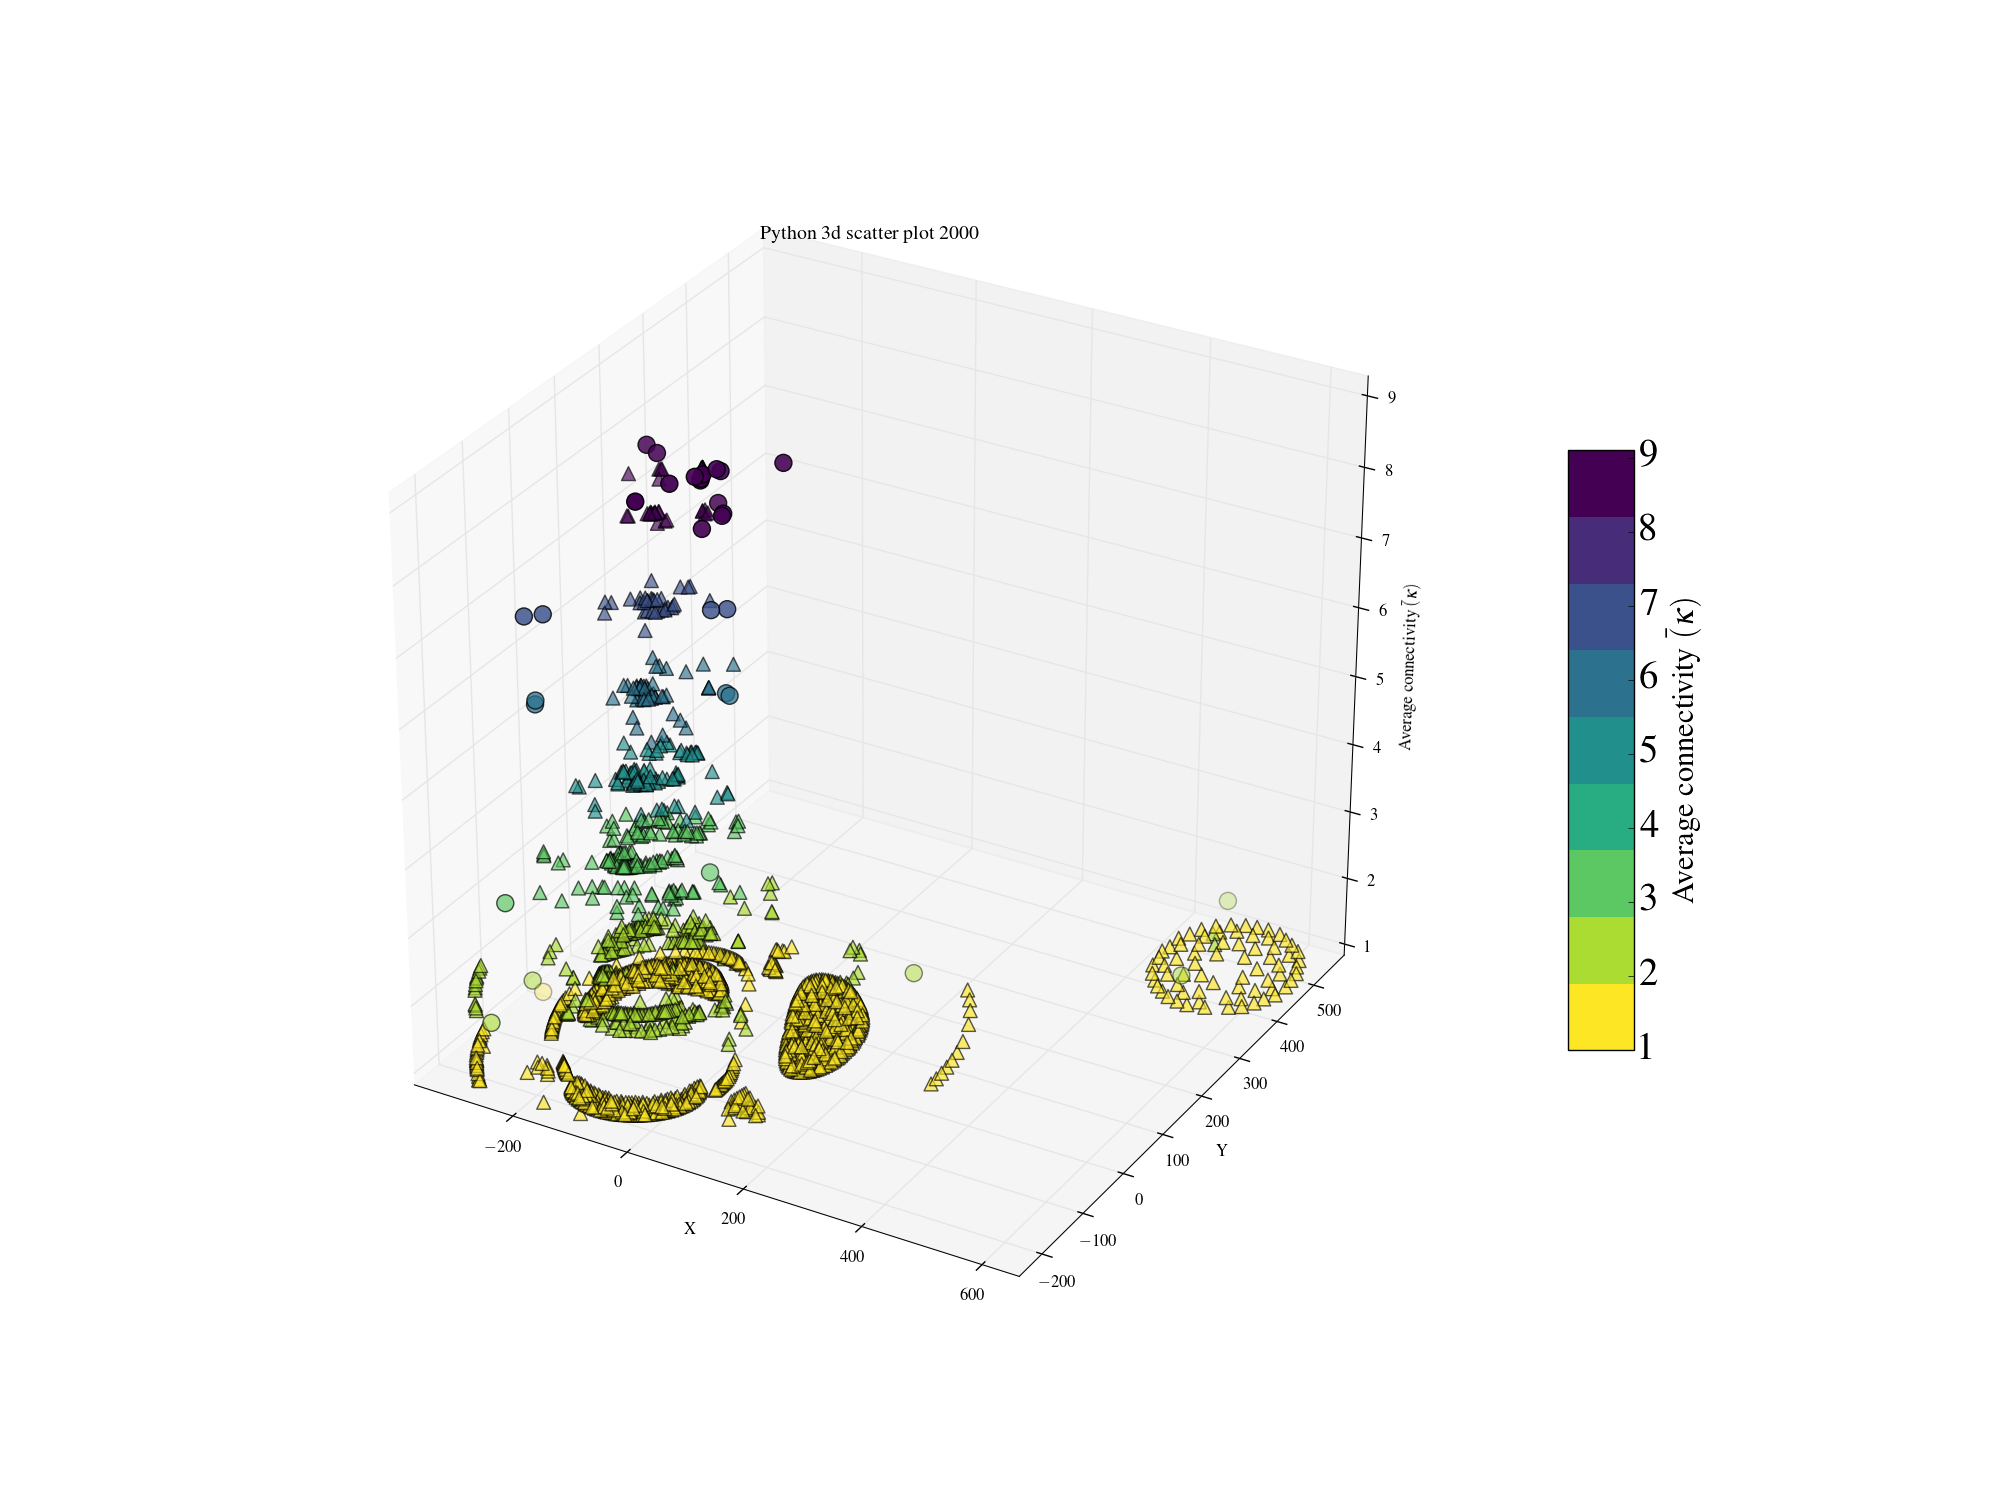
\includegraphics[scale=0.23]{figures/3d_scatter_python_2000}
}
\hspace{.01in}
\subfloat[Null model Python network 2000]{
\label{fig:s3d_null_python_2000}
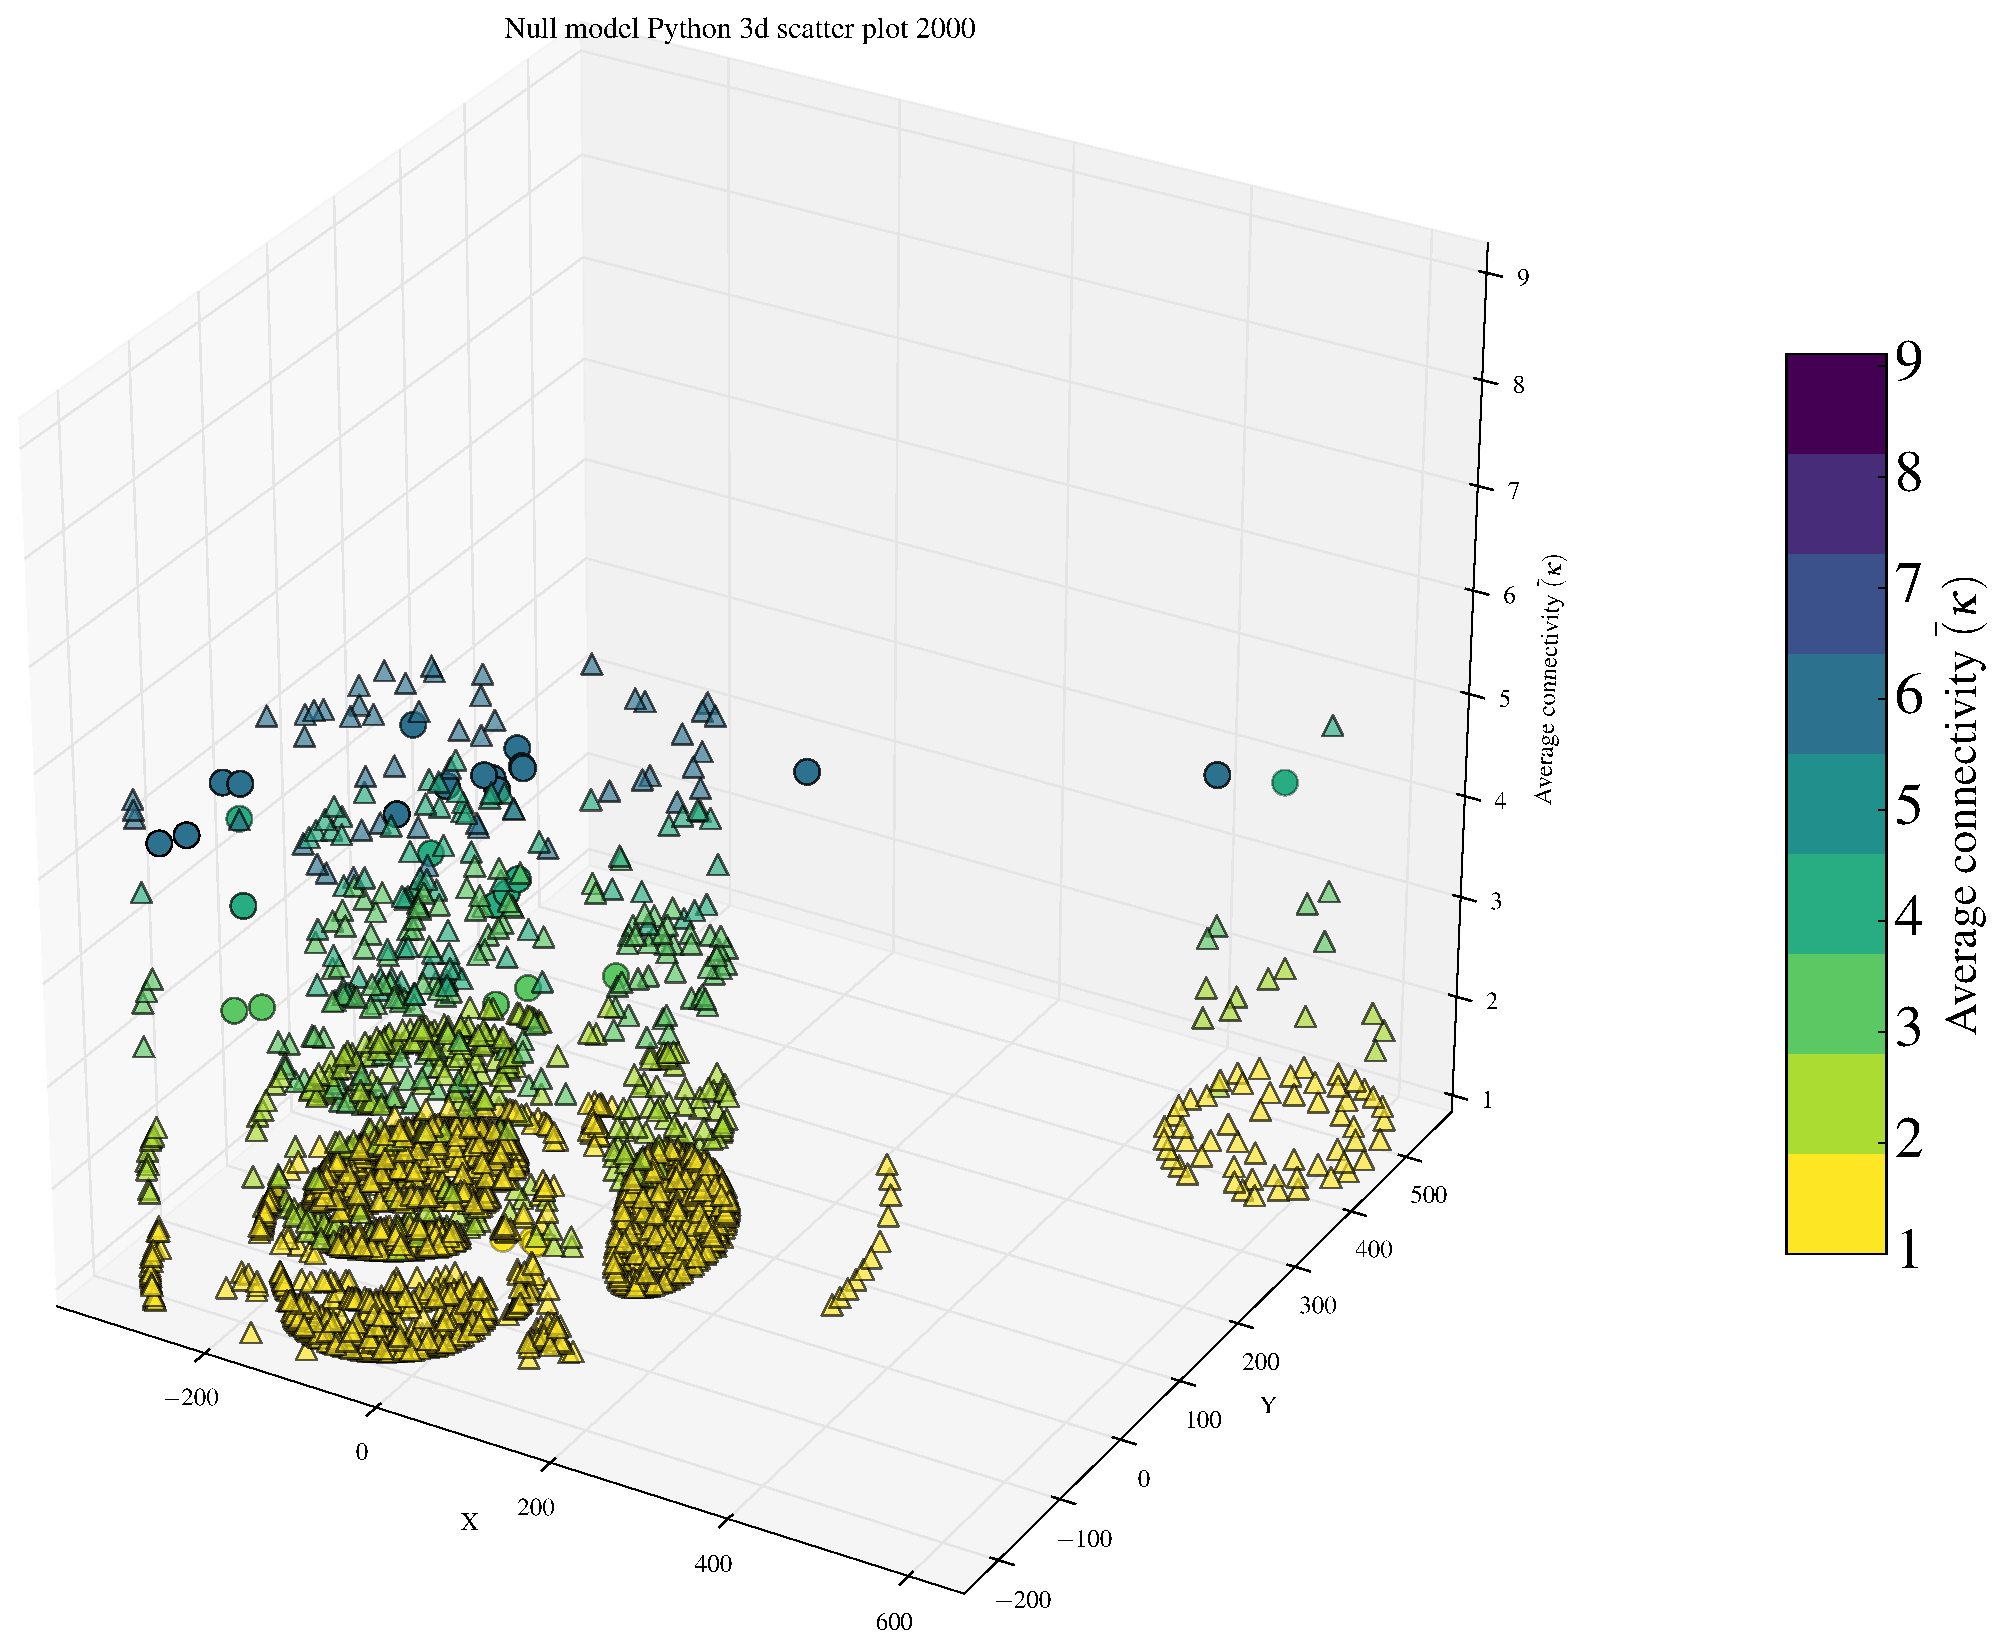
\includegraphics[scale=0.23]{figures/3d_scatter_python_2000_null}
}

\subfloat[Actual Python network 2004]{
\label{fig:s3d_actual_python_2004}
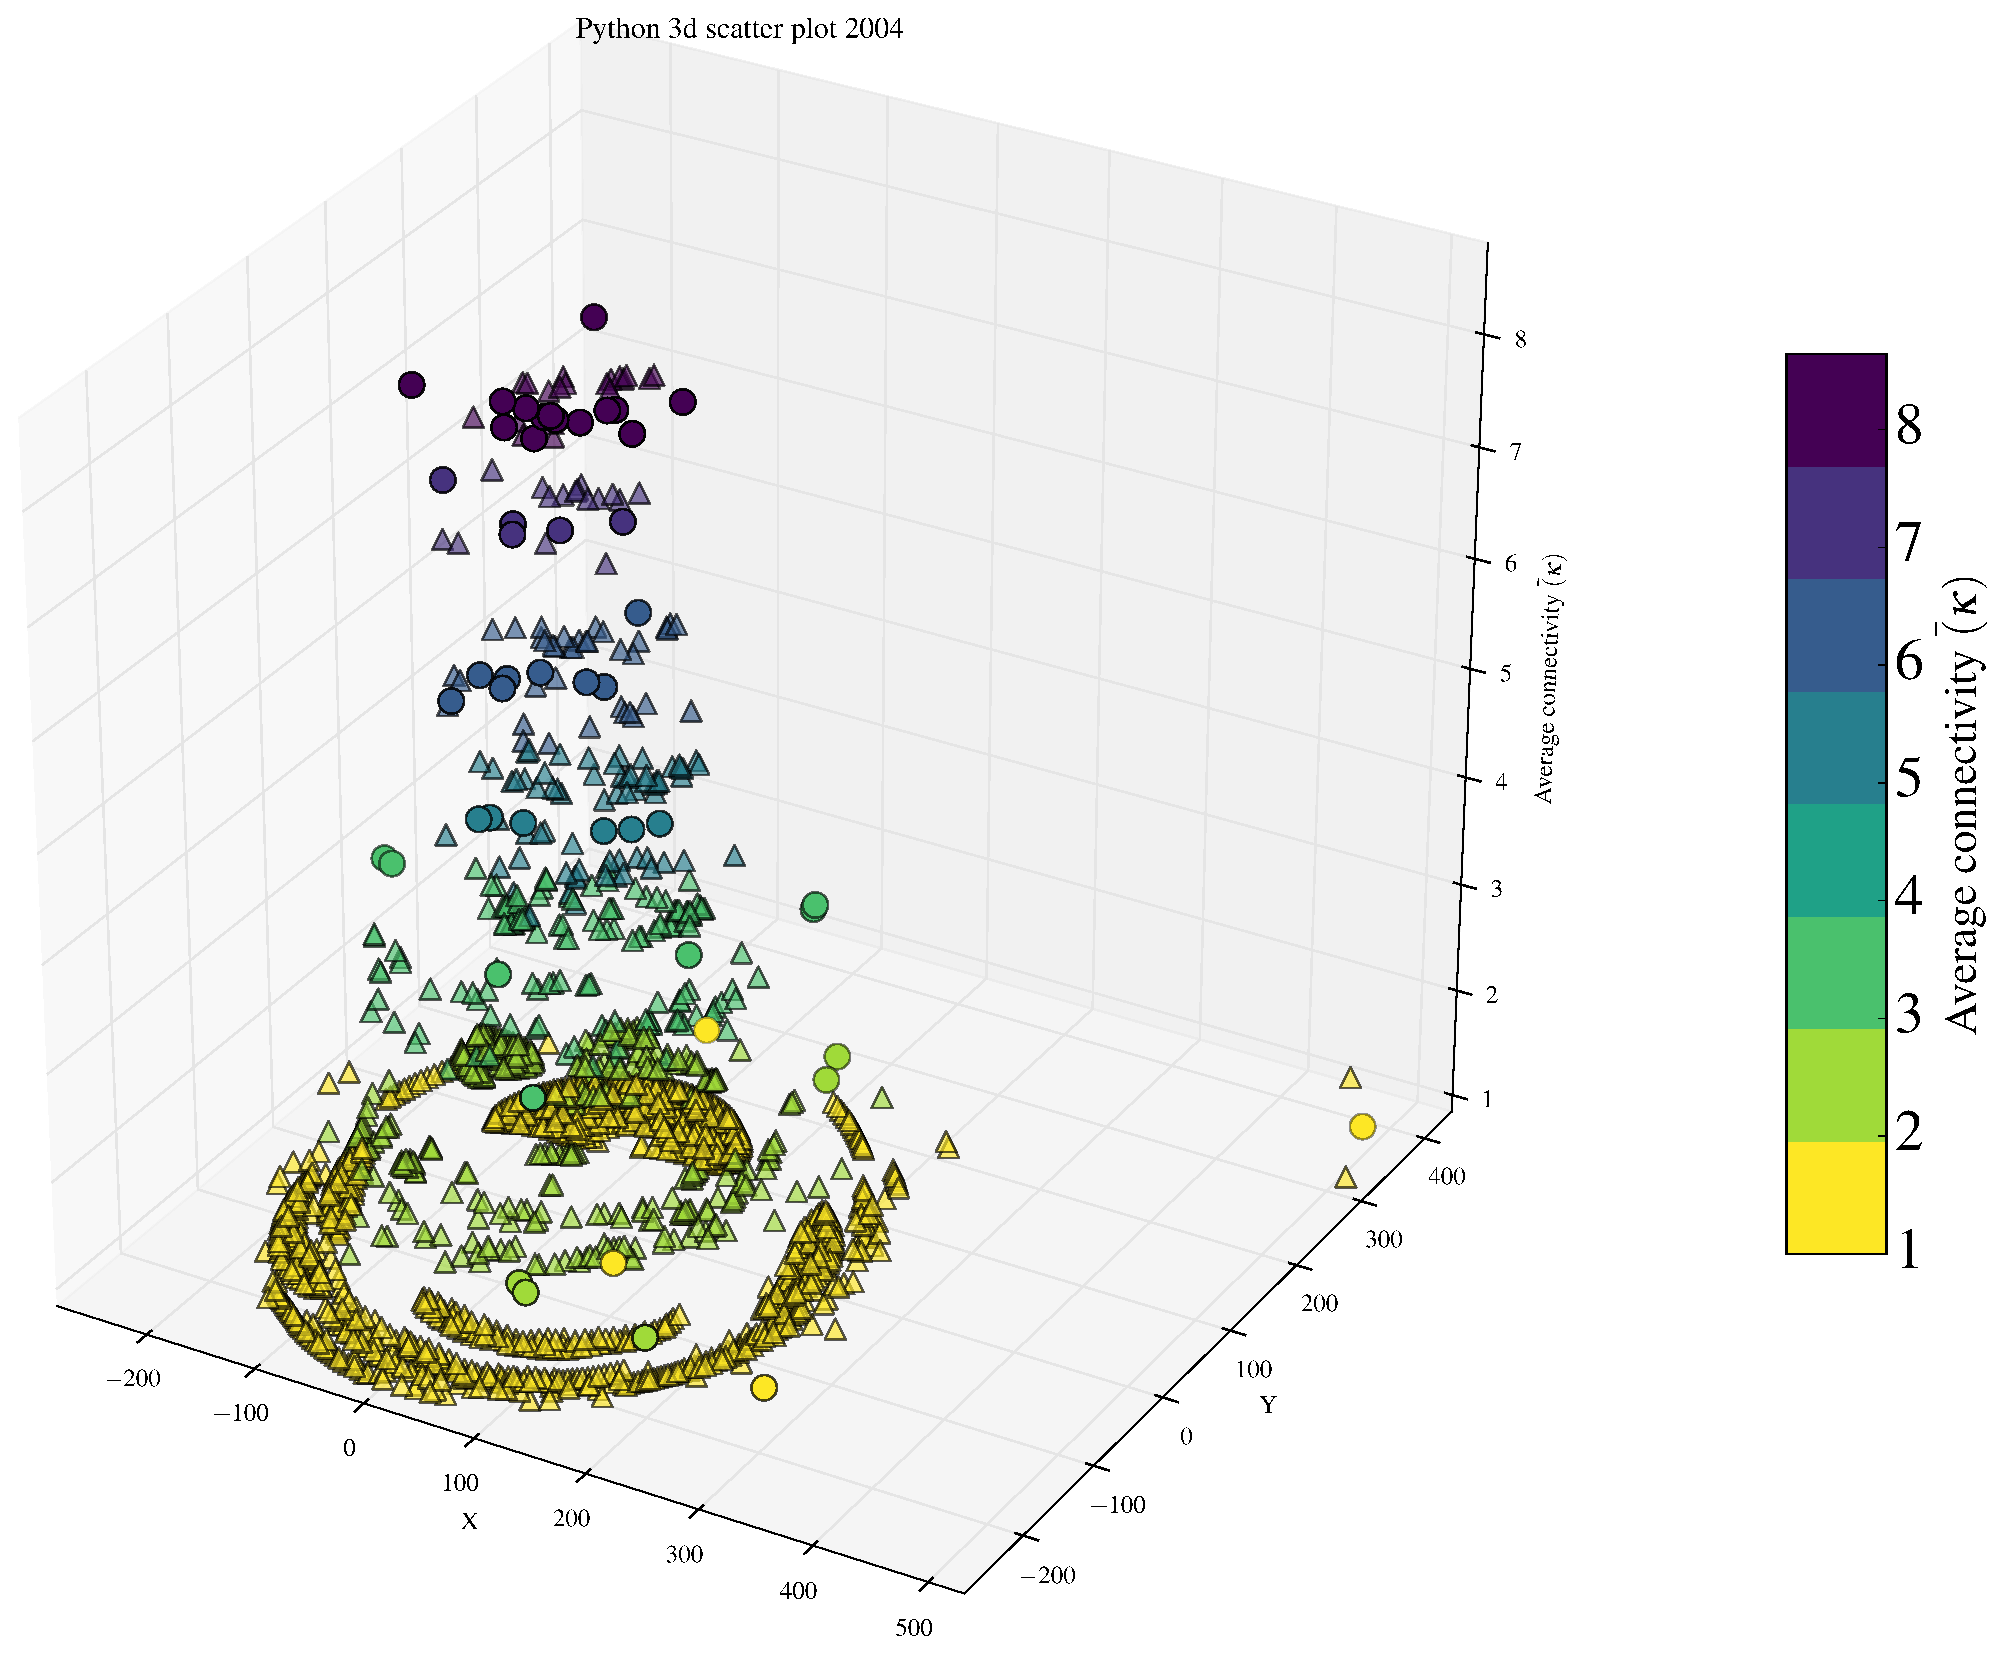
\includegraphics[scale=0.23]{figures/3d_scatter_python_2004}
}
\hspace{.01in}
\subfloat[Null model Python network 2004]{
\label{fig:s3d_null_python_2004}
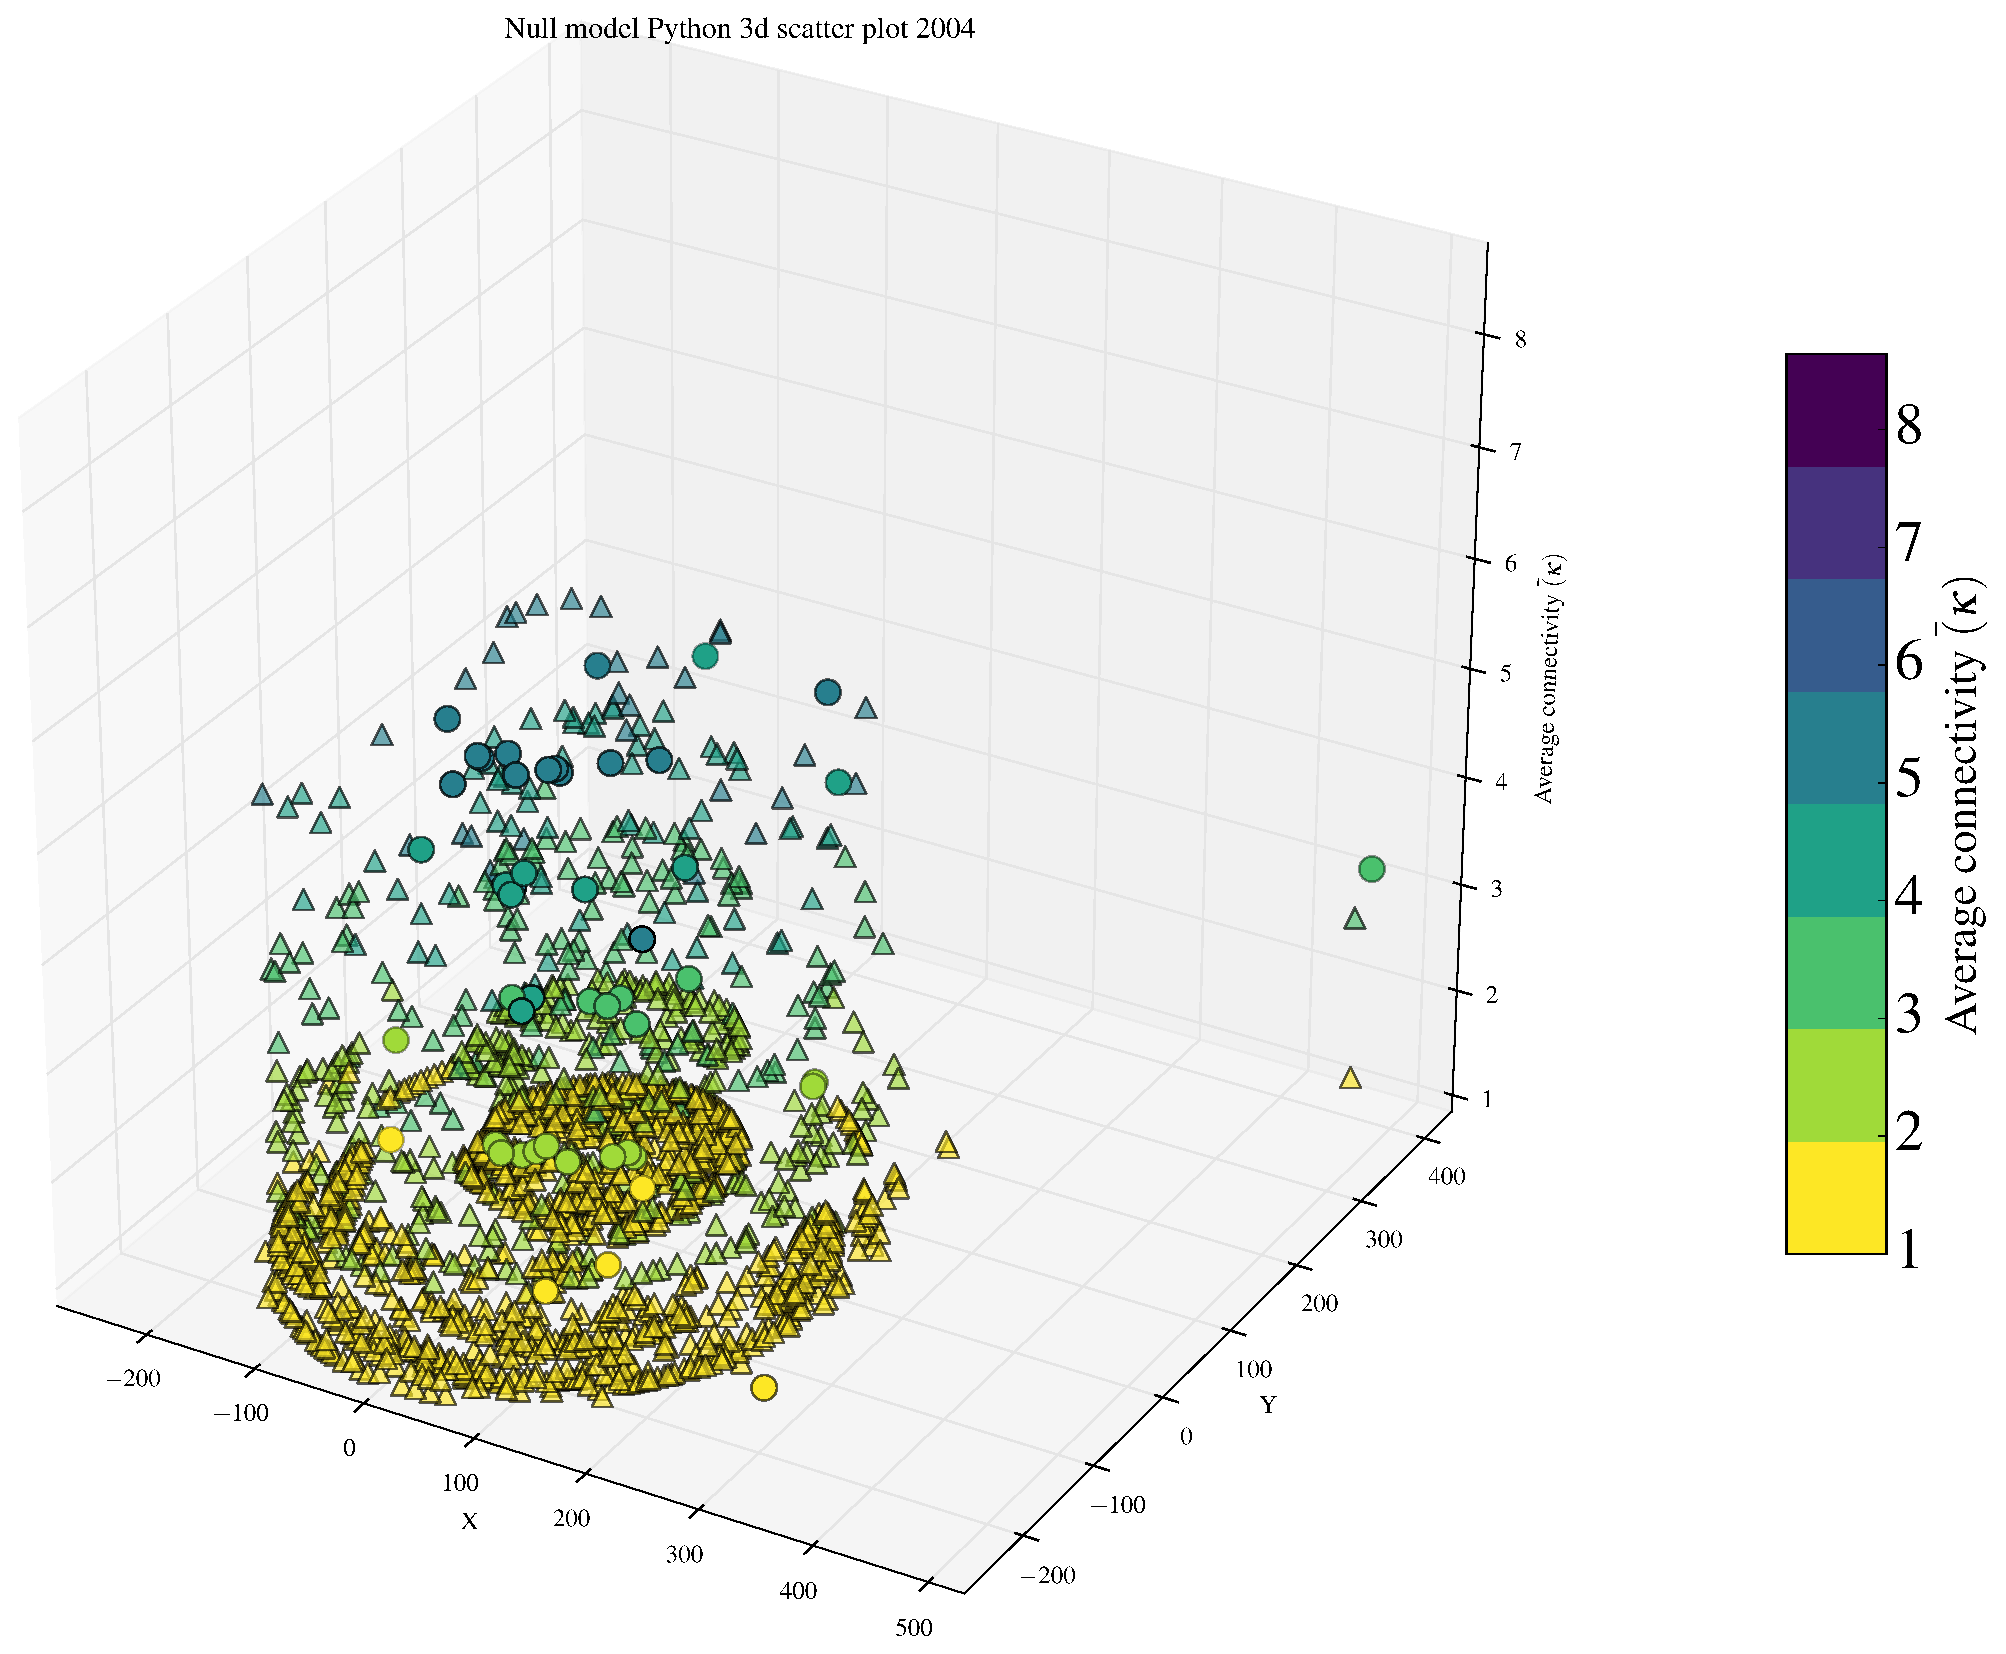
\includegraphics[scale=0.23]{figures/3d_scatter_python_2004_null}
}

\subfloat[Actual Python network 2013]{
\label{fig:s3d_actual_python_2013}
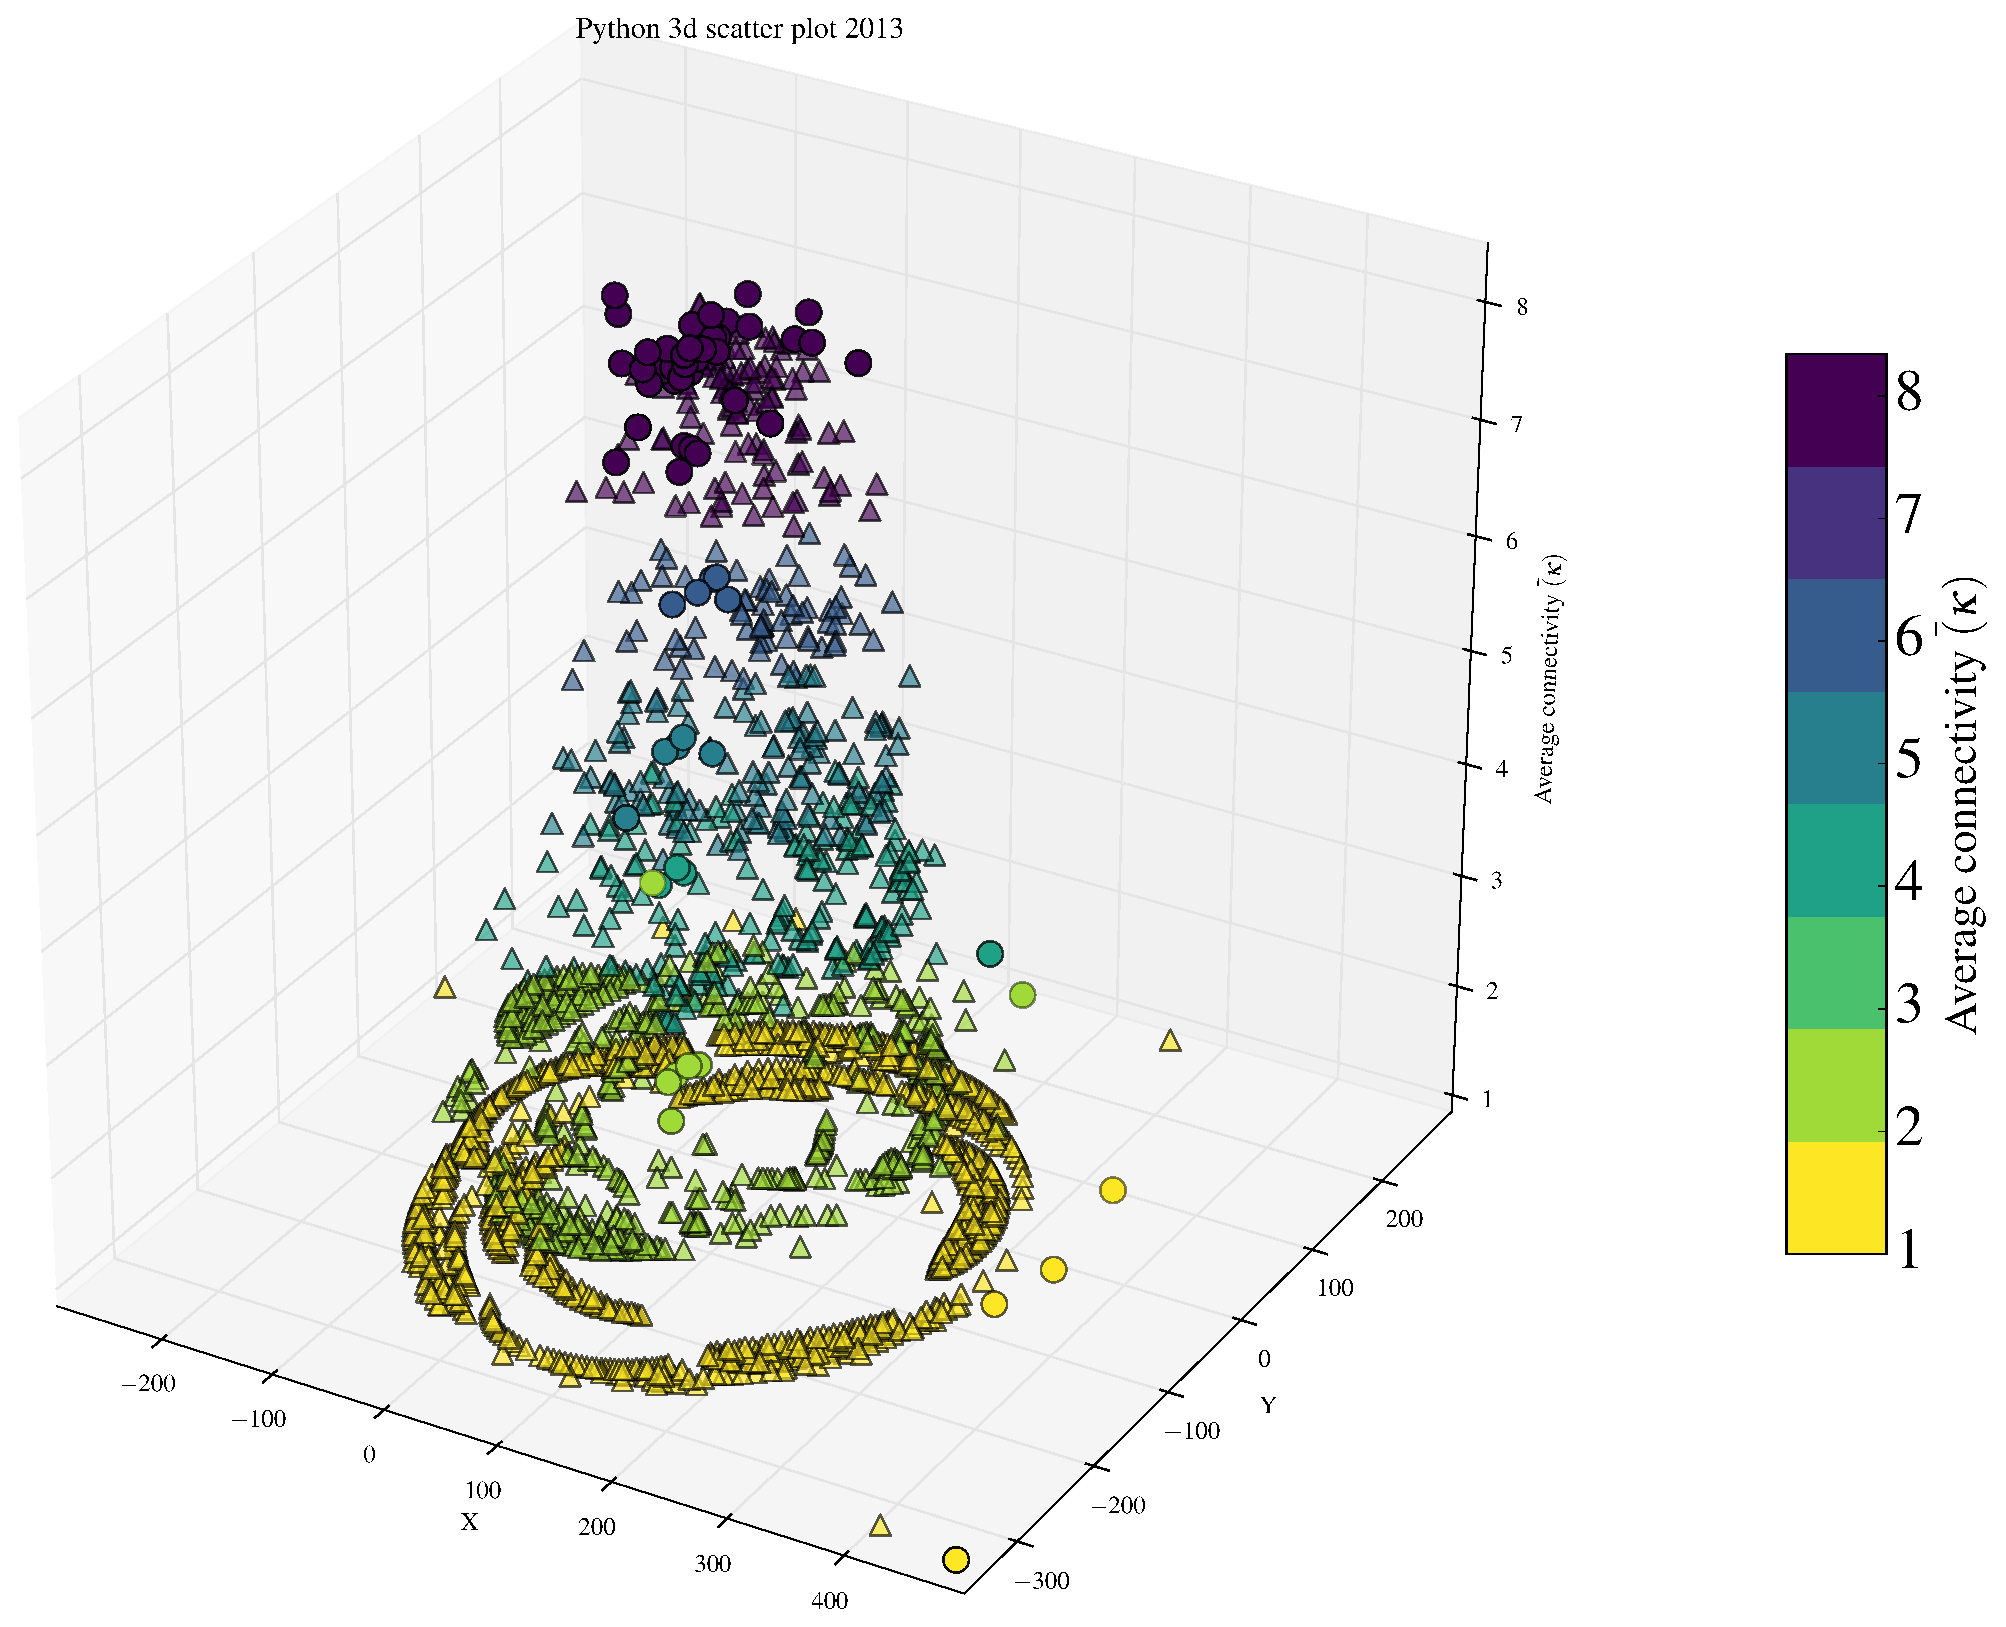
\includegraphics[scale=0.23]{figures/3d_scatter_python_2013}
}
\hspace{.01in}
\subfloat[Null model Python network 2013]{
\label{fig:s3d_null_python_2013}
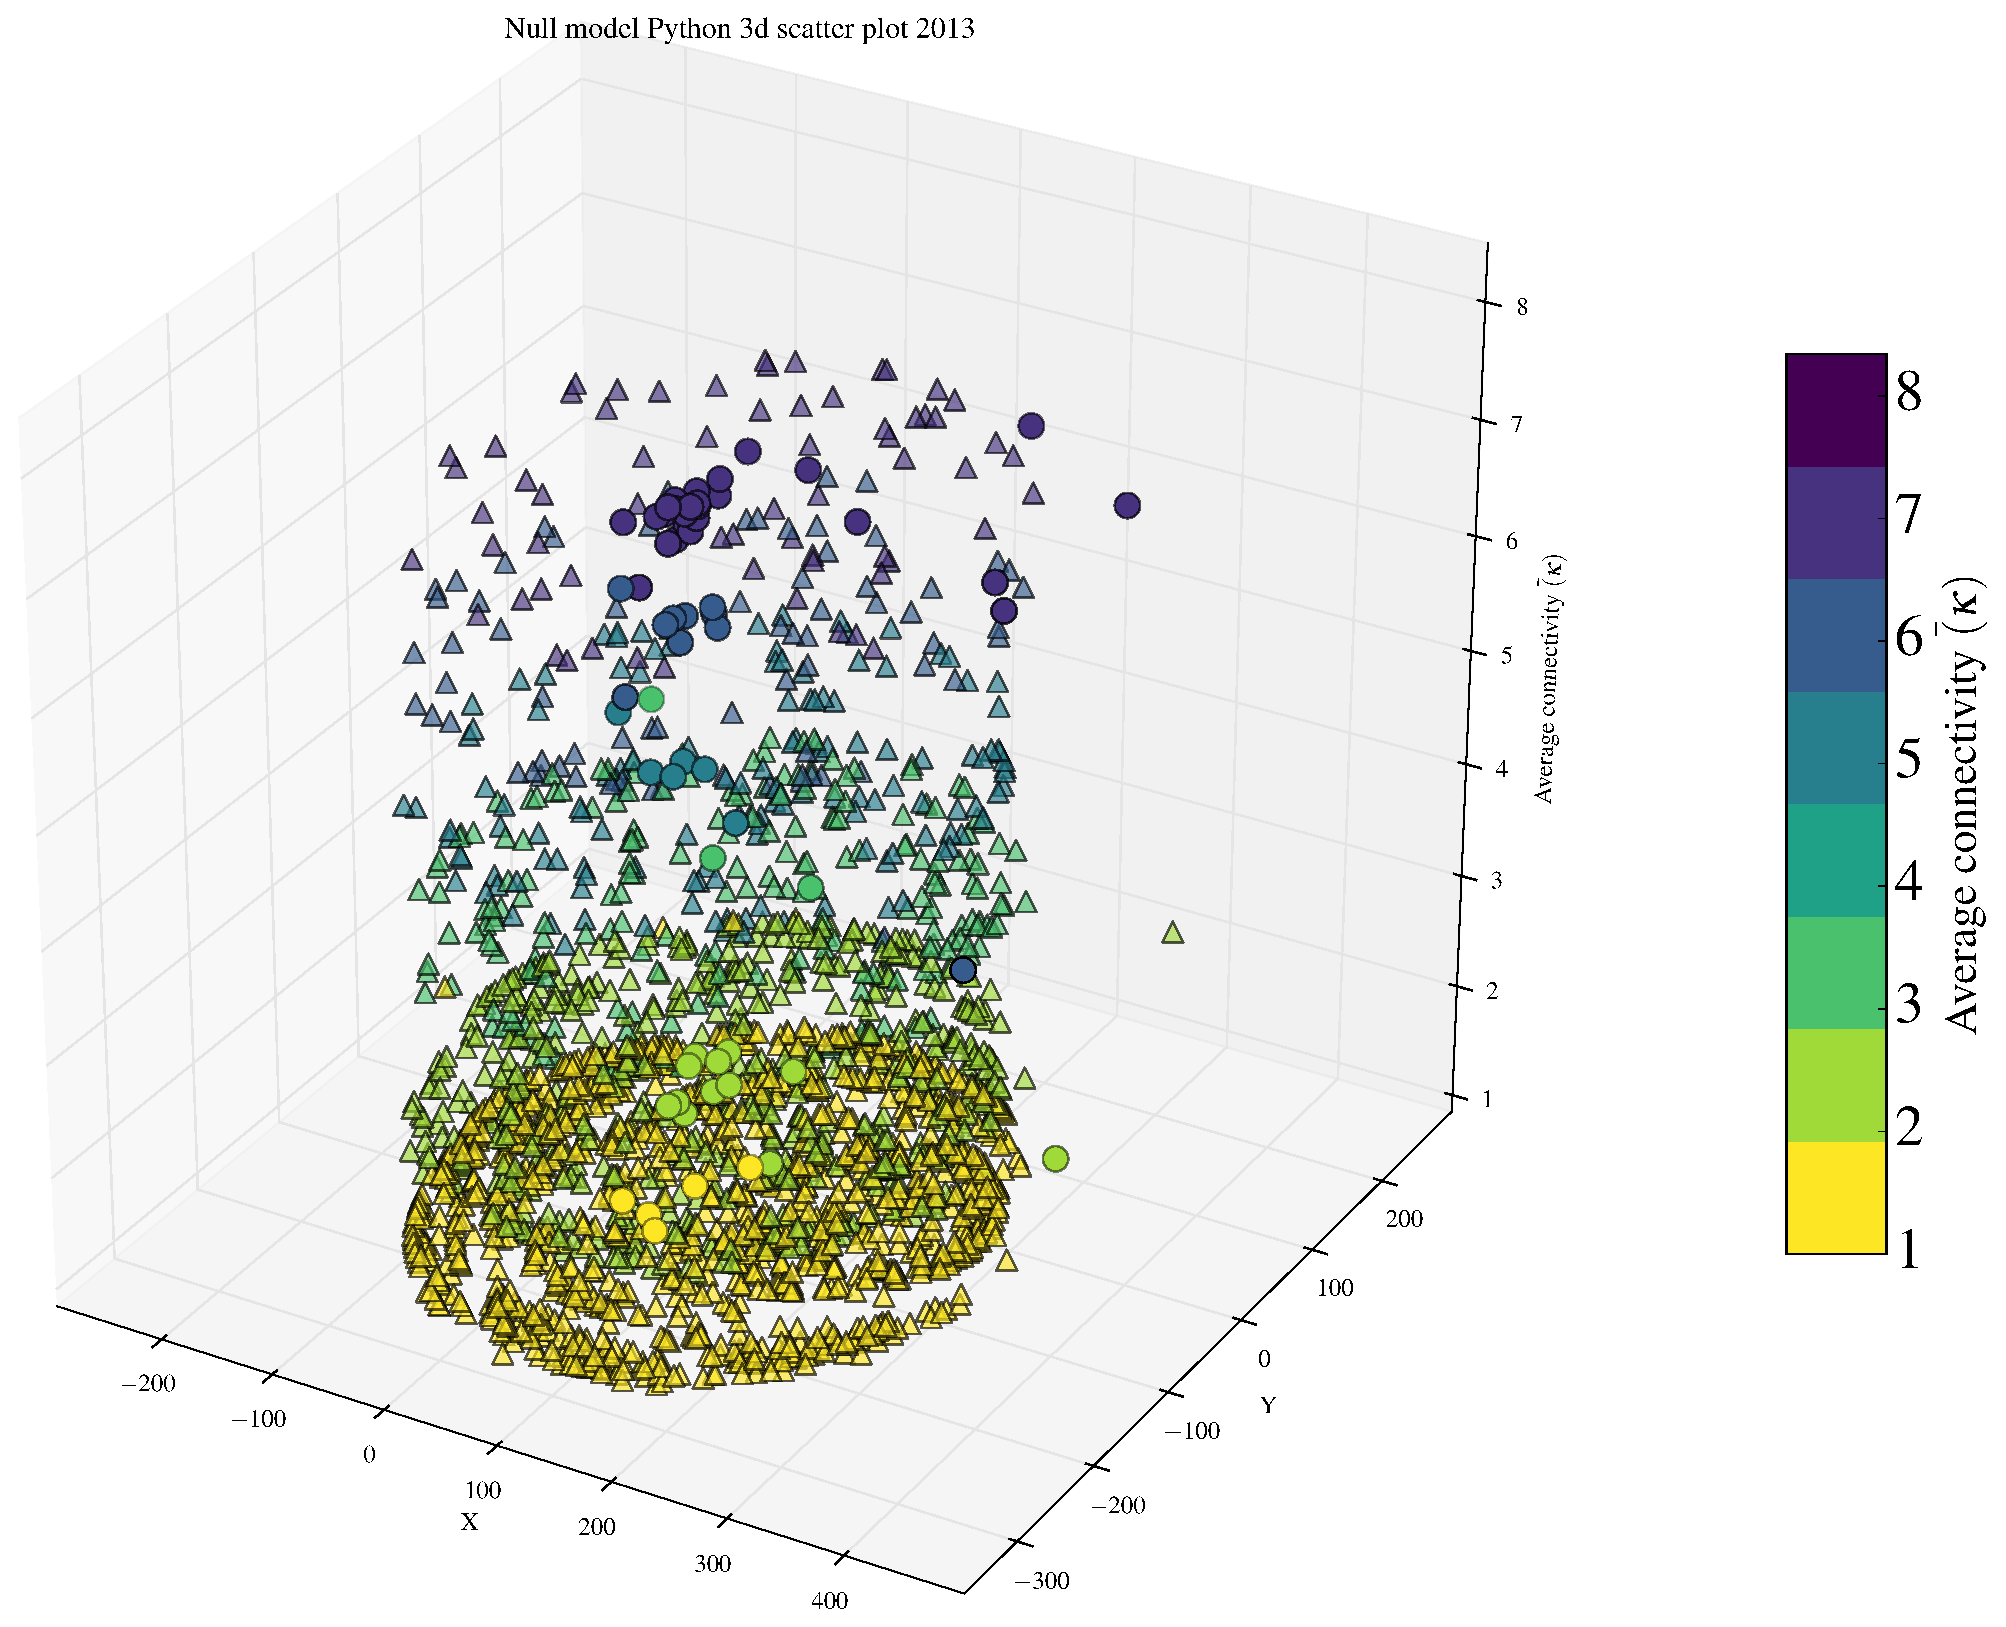
\includegraphics[scale=0.23]{figures/3d_scatter_python_2013_null}
}

\caption[Python average connectivity three-dimensional scatter plots.]{Python average connectivity three-dimensional scatter plots for actual networks and their random null models counterparts. X and Y are the positions determined by the Kamada-Kawai layout algorithm. The vertical dimension is average connectivity. Each mark is a node of the network as two-mode networks they contain both programs (triangles) and developers (circles).}
\label{fig:python-s3d}
\end{figure}

Finally the last two columns of table \ref{str_cohesion_python} clearly show that the actual cooperation networks have higher connectivity levels at the top of the connectivity hierarchy than their random counterparts. From 2000 to 2010 ---excluding again 1999--- the difference is between two and three hierarchy levels but in the last years. For instance, in 2008 the actual cooperation network has a subroup with 2.2\% percent of nodes that forms a 10-component, which means that we need to remove 10 nodes from that group in order to disconnect it ---or equivalently, we have to remove 10 nodes to destroy all relational paths between any two nodes in that group. The random network used as a null model for that year has only one subgroup that has connectivity 7.

These high connectivity $k$-components only have a very small percentatge of all the nodes in the cooperation network (between 1 and 5.8\% of all nodes), but as we will see in the next chapter, they play a key role in terms of their contribution to the project measured in the number of source code lines added to the files that form the code base of the Python language. Also, at a theoretical level, these subgroups with high connectivity 

As discussed in chapter \ref{structural_cohesion}, it's useful to visualize the $k$-component hierarchy of the cooperation networks in order to gain a better understanding of their structure and to be able to easily compare between the actual networks and their random counterparts. Figure \ref{fig:python-s3d} shows Python cooperation networks for years 2000, 2004 and 2013 along with their random counterparts using the novel visualization technique that we presented in chapter \ref{structural_cohesion} and on our own publication \citep{torrents:2015}.

Using this novel visualization techique it's easy to see the differences in the hierarchy structure between the actual cooperation networks and their random counterparts. Actual networks not only have a higher connectivity levels at the top but their hirearchical structure is more steep than their random chierarchies, which thend to have nodes more evently distributed between connectivity levels and thus tend to be flatter hierarchies precisely because edges in random network are also more evently distributed among nodes than in their actual counterparts.

After examining the tables and the figures for the Python cooperation networks we can conclude that the cooperation networks of the Python project fit nicely with the structural cohesion model. And, as explained above, also fit well the small world model. This allows us to assess that they indeed are a case of what we named the cohesive small world model.

\begin{table}[H]
\begin{center}
\begin{tabular}{|c|c|c|c|c|c|c|c|}
\hline
Years&Nodes&GC&Random GC&GBC&Random GBC&maximum $k$&Random max $k$\\
\hline
1999&3,259&66.6\%&83.4\%&9.4\%&11.4\%&3 (0.2\%)&2 (11.4\%)\\
2000&3,593&52.5\%&77.8\%&7.0\%&10.7\%&3 (0.2\%)&2 (10.7\%)\\
2001&5,943&71.6\%&86.4\%&13.9\%&17.5\%&3 (0.1\%)&2 (17.5\%)\\
2002&6,857&72.4\%&88.1\%&12.7\%&17.0\%&4 (0.2\%)&2 (17.0\%)\\
2003&7,276&75.6\%&89.5\%&14.8\%&20.2\%&5 (0.2\%)&2 (20.2\%)\\
2004&7,984&78.4\%&94.4\%&22.1\%&27.7\%&5 (0.2\%)&2 (27.7\%)\\
2005&8,328&83.8\%&94.4\%&26.1\%&31.3\%&4 (0.5\%)&3 (4.5\%)\\
2006&9,599&84.2\%&96.7\%&33.7\%&39.0\%&4 (0.6\%)&3 (8.4\%)\\
2007&9,471&86.5\%&96.1\%&35.6\%&40.7\%&4 (0.2\%)&3 (8.6\%)\\
2008&10,662&87.2\%&96.4\%&34.3\%&40.3\%&4 (0.6\%)&3 (7.5\%)\\
2009&11,336&89.4\%&96.1\%&35.7\%&42.3\%&5 (0.4\%)&3 (8.2\%)\\
2010&10,515&86.9\%&95.5\%&32.7\%&39.8\%&5 (0.2\%)&3 (5.1\%)\\
2011&12,362&87.7\%&95.0\%&30.6\%&36.0\%&5 (0.3\%)&3 (5.3\%)\\
2012&11,904&87.1\%&95.0\%&31.0\%&36.7\%&4 (0.1\%)&3 (2.3\%)\\
\hline
\end{tabular}
\caption{Structural Cohesion metrics for debian networks.}
\label{str_cohesion_debian}
\end{center}
\end{table}



Regarding the Debian project, table \ref{str_cohesion_debian}, reports the structural cohesion analysis of their connectivity structure. As we can see the percentage of nodes of cooperation networks that form the giant component is smaller than the percentage in their random counterparts in all years under analsysis. As explained above, for low connectivity levels the size for the giant components and bicomponents are an upper bound for the actual networks \citep{moody:2004}. In that sense, Python cooperation networks examined above are exceptional in that they equal or even surpass their random counterparts for low connectivity levels.

In the case of Debian networks we see an steady increase of the relative size of the giant component from 1999 to 2005, where the percentage stabilizes arround eighty percent of the total nodes. However their random network counterparts grow similarly but there are approximately fifteen percent more nodes in the random giant components than in actual networks, stabilizing around 95\% of the total nodes after 2005. For the case of giant bicomponents (column ``GBC''), we see a similar picture than with the giant components: an steady increment of the relative size of bicomponents until 2006, where their relative size stabilizes arround 30\% of the nodes of the network wuth a peak of 34\% in 2009. During all the period analyzed the random configuration model networks have a relative size of their giant bicomponent approximately 7\% higher than their actual counterparts, also peaking in 2009 with 40\% of the nodes.   

For the higher connectivity levels, reported in the last two columns of the table, we can see that the actual cooperation networks have higher connectivity levels not present in the random configuration models used as null models. The difference in connectivty levels tends to increase in the later part of the period analyzed, where actual cooperation networks have $5$-components ---that is subgroups from which we have to remove five nodes in order to disconnect them--- while random networks in all period analyzed have only $3$-components as thei higher connectivity levels.

The number of nodes in the high connectivity subgroups in the actual cooperation networks is very low: less than 1\% of all nodes. Note however that because of the total number of nodes in the Debian cooperation networks is quite big these subgroups are formed between 40 and 60 nodes. 

In order to gain a better understanding of the shape of the hirearchical structure of these cooperation networks, and to compare them to their random counterparts we have to look at figure \ref{fig:debian-s3d} where three dimensional scatter plots are shown for Debian cooperation networks for years 2000, 2004, and 2011, along with their random counterparts. Similarly to the Python cooperation networks, actual networks have a more steep connectivity hierarchy than their random counterparts because, on the one hand, they have nodes in higher connectivity levels that are not present in the random configuration models and, on the other hand, nodes in actual cooperation networks are less evently distributed between connectivity levels. Thus we can conclude that Debian cooperation networks also correctly fit the structural cohesion model. And therefore they also conform to the model that we named cohesive small world.

The analysis presented in this chapter shows that the cooperation networks of both Debain and Python projects can be modelled using our proposed cohesive small world model. It is intersting to note that they also show significative differences because Debain cooperation networks basculate more to the small world end of the model, while Python cooperation networks basculate more towards the structural cohesion end of the model. As discussed above, their difference in terms of modularity of the product that they are building ---an Operating System versus a Programming language--- impacts their respective production processes. Debian's subgroups tend to work more independently from each other than Python's subgroups, as shown by the fact that Debian cooperation networks exhibit a higher degree of smallworldiness; while Python's networks are more structurally cohesive as shown by their sharper and steep connectecty hierarchy.

The next step in our analysis is to analyze the contribution levels of developers in both projects in the different levels of the connectivity hierarchy in order to a assess the actual impact of this hierarchy of the respective cooperation networks in the production process of both projects. This is the focus of the next chapter.


\begin{figure}[p]
%\centering
\subfloat[Actual Debian network 2000]{
\label{fig:s3d_actual_debian_2000}
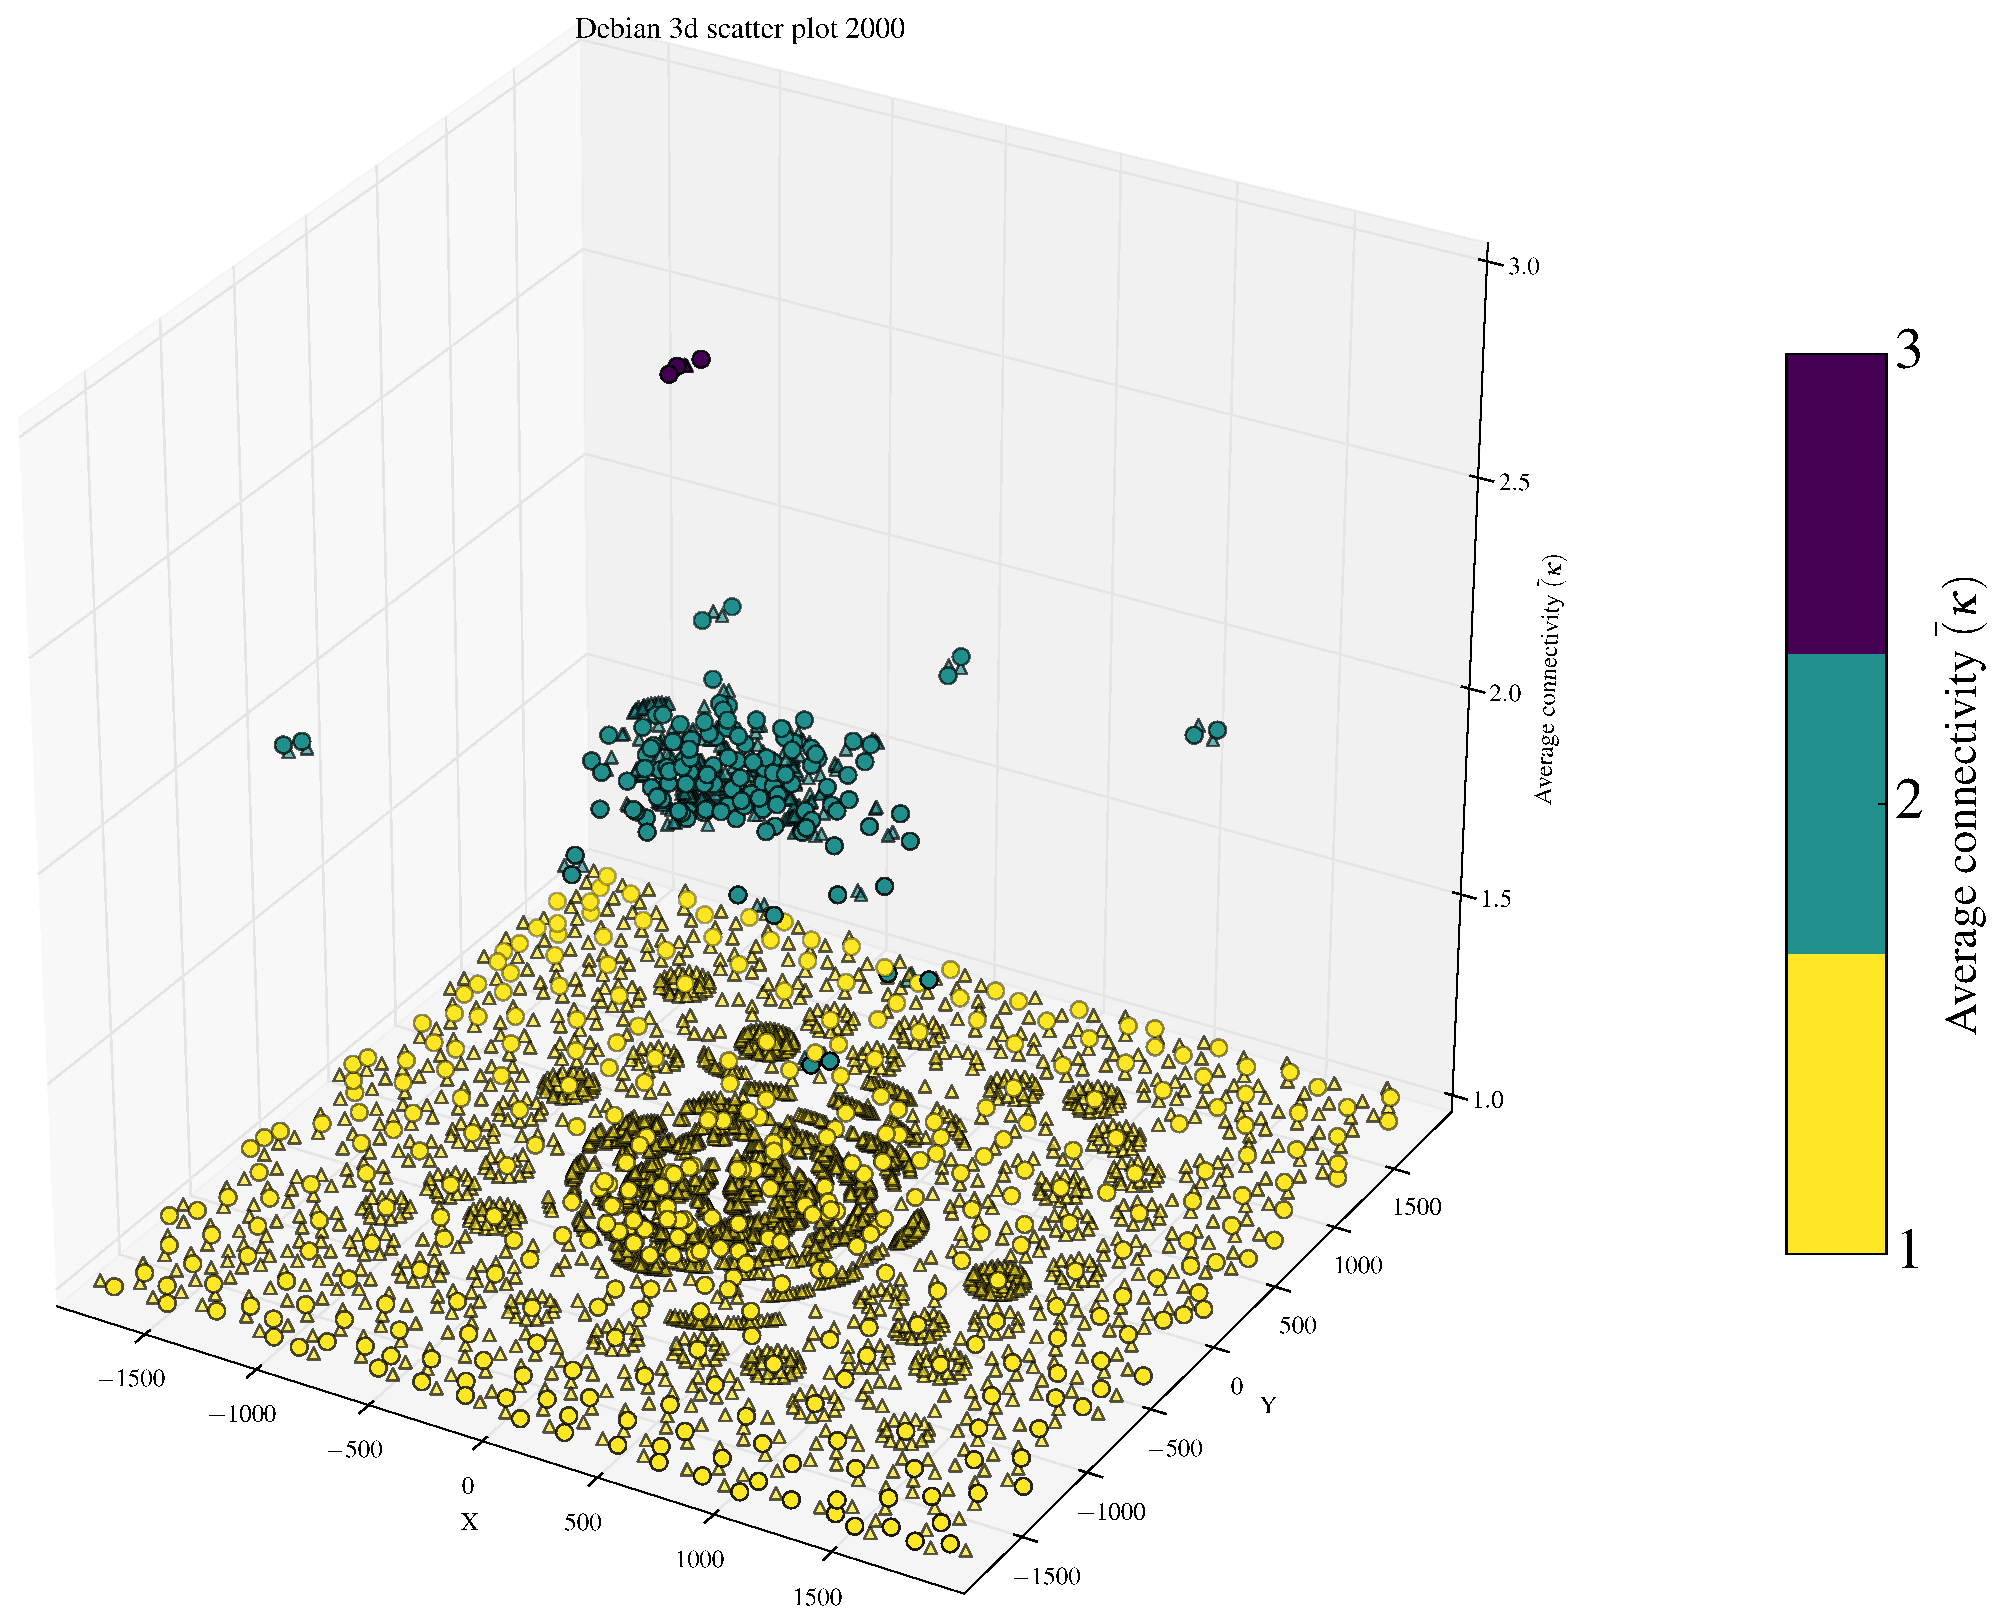
\includegraphics[scale=0.23]{figures/3d_scatter_debian_2000}
}
\hspace{.01in}
\subfloat[Null model Debian network 2000]{
\label{fig:s3d_null_debian_2000}
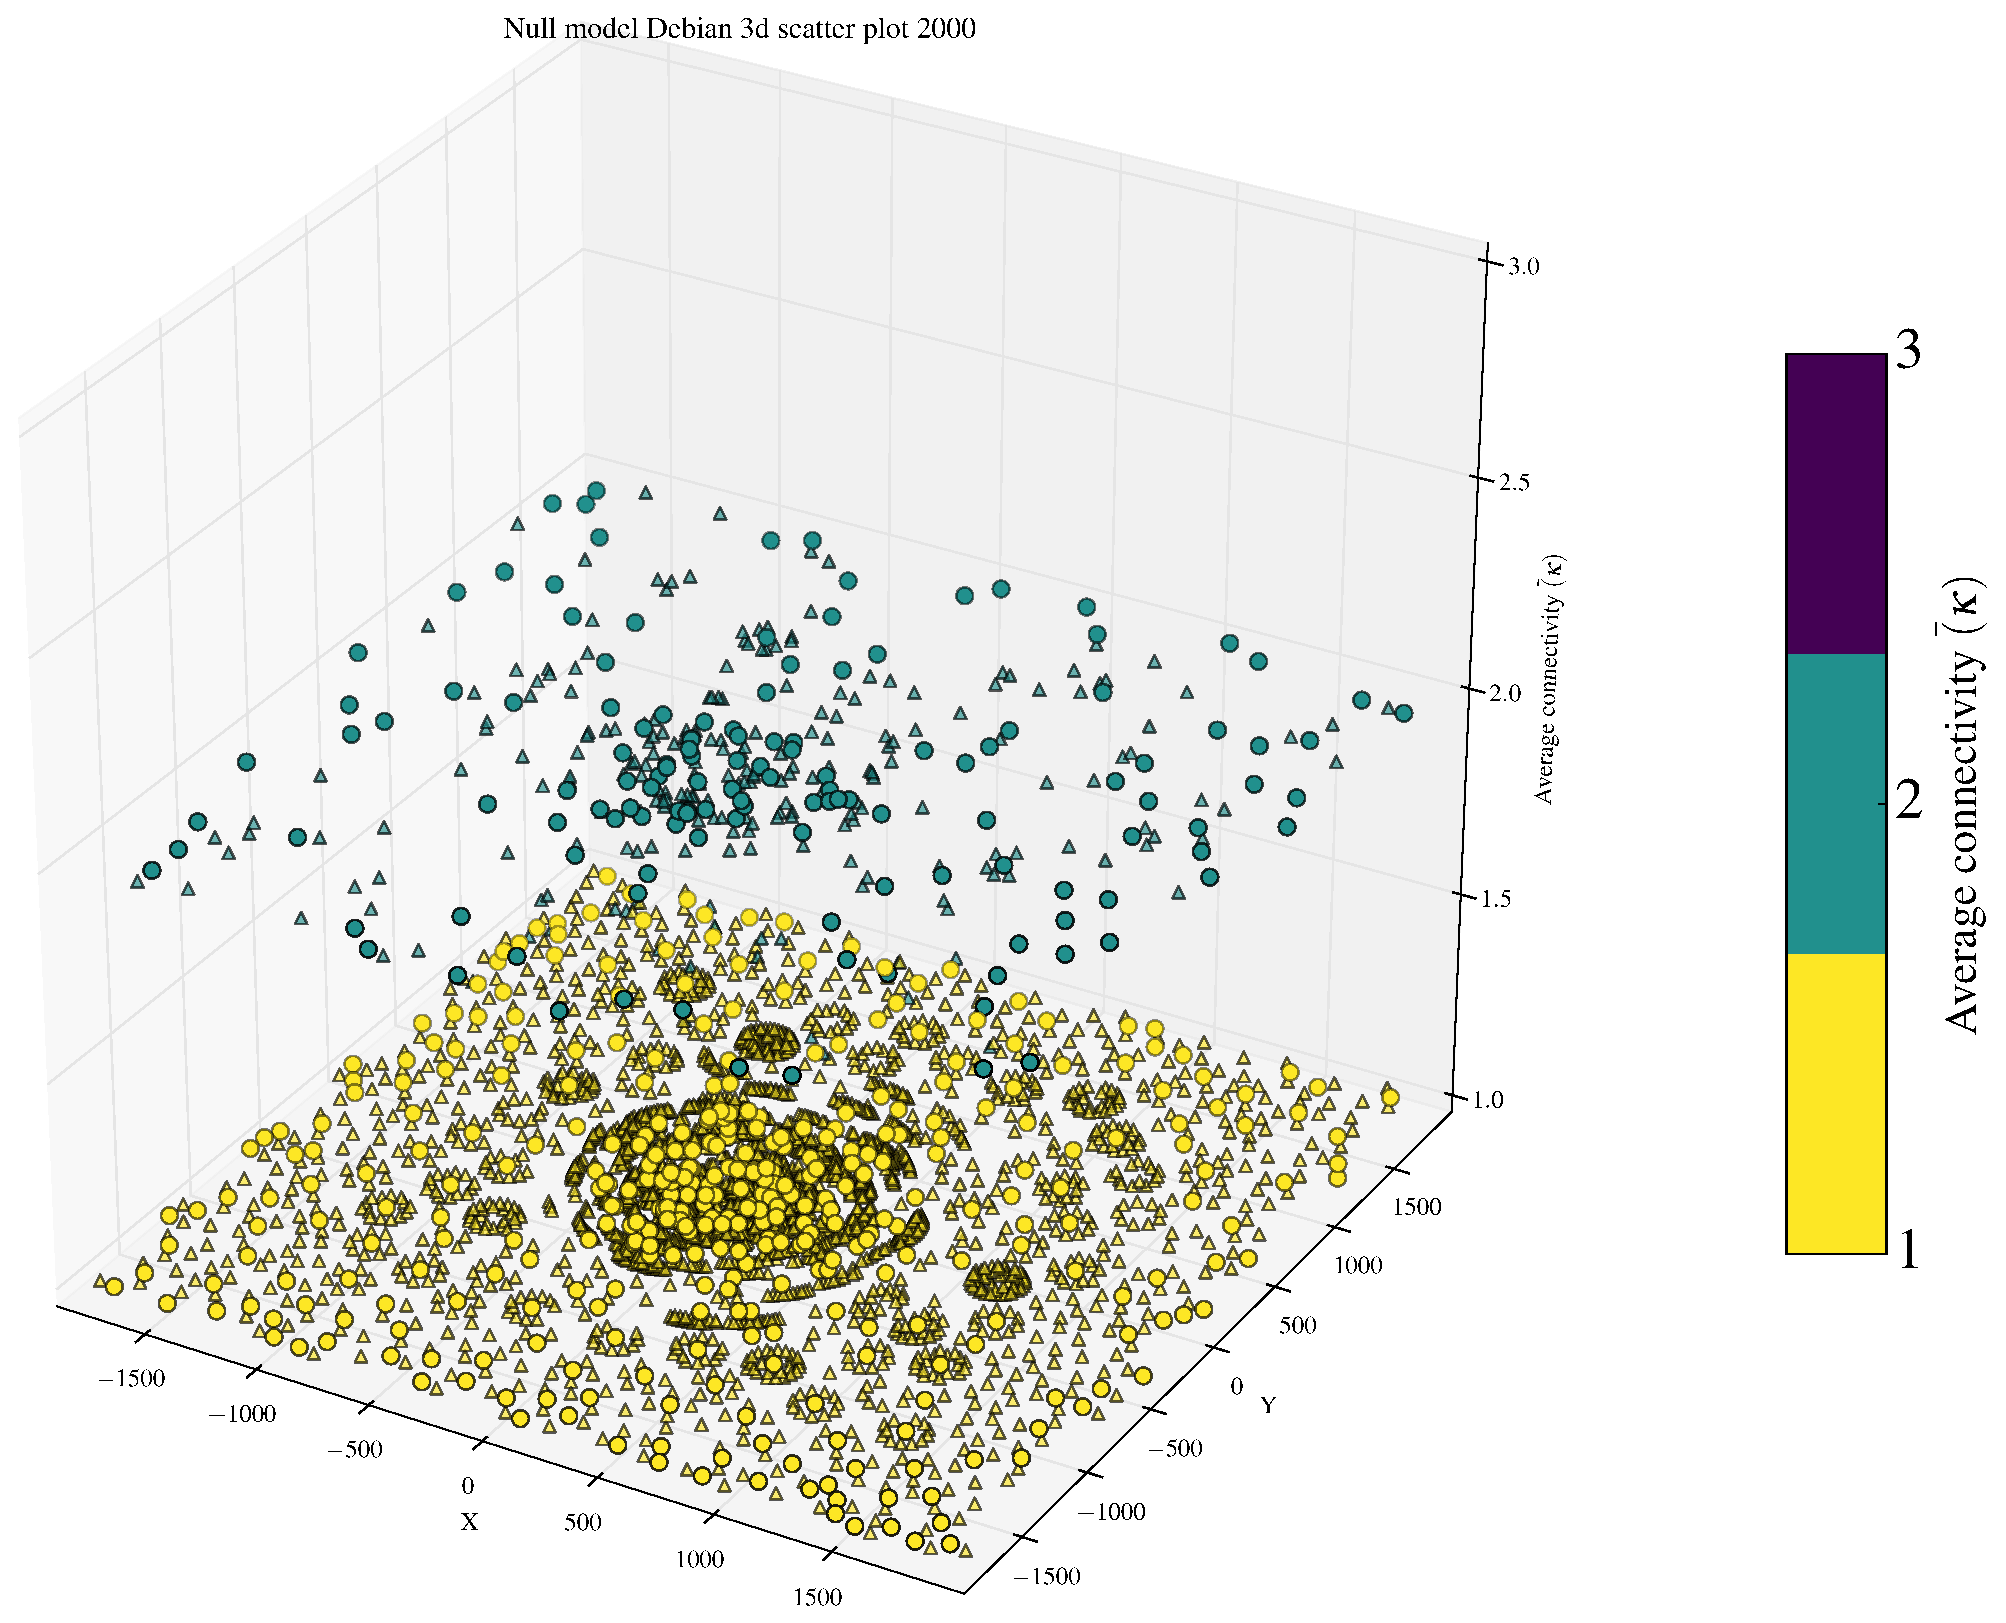
\includegraphics[scale=0.23]{figures/3d_scatter_debian_2000_null}
}

\subfloat[Actual Debian network 2004]{
\label{fig:s3d_actual_debian_2004}
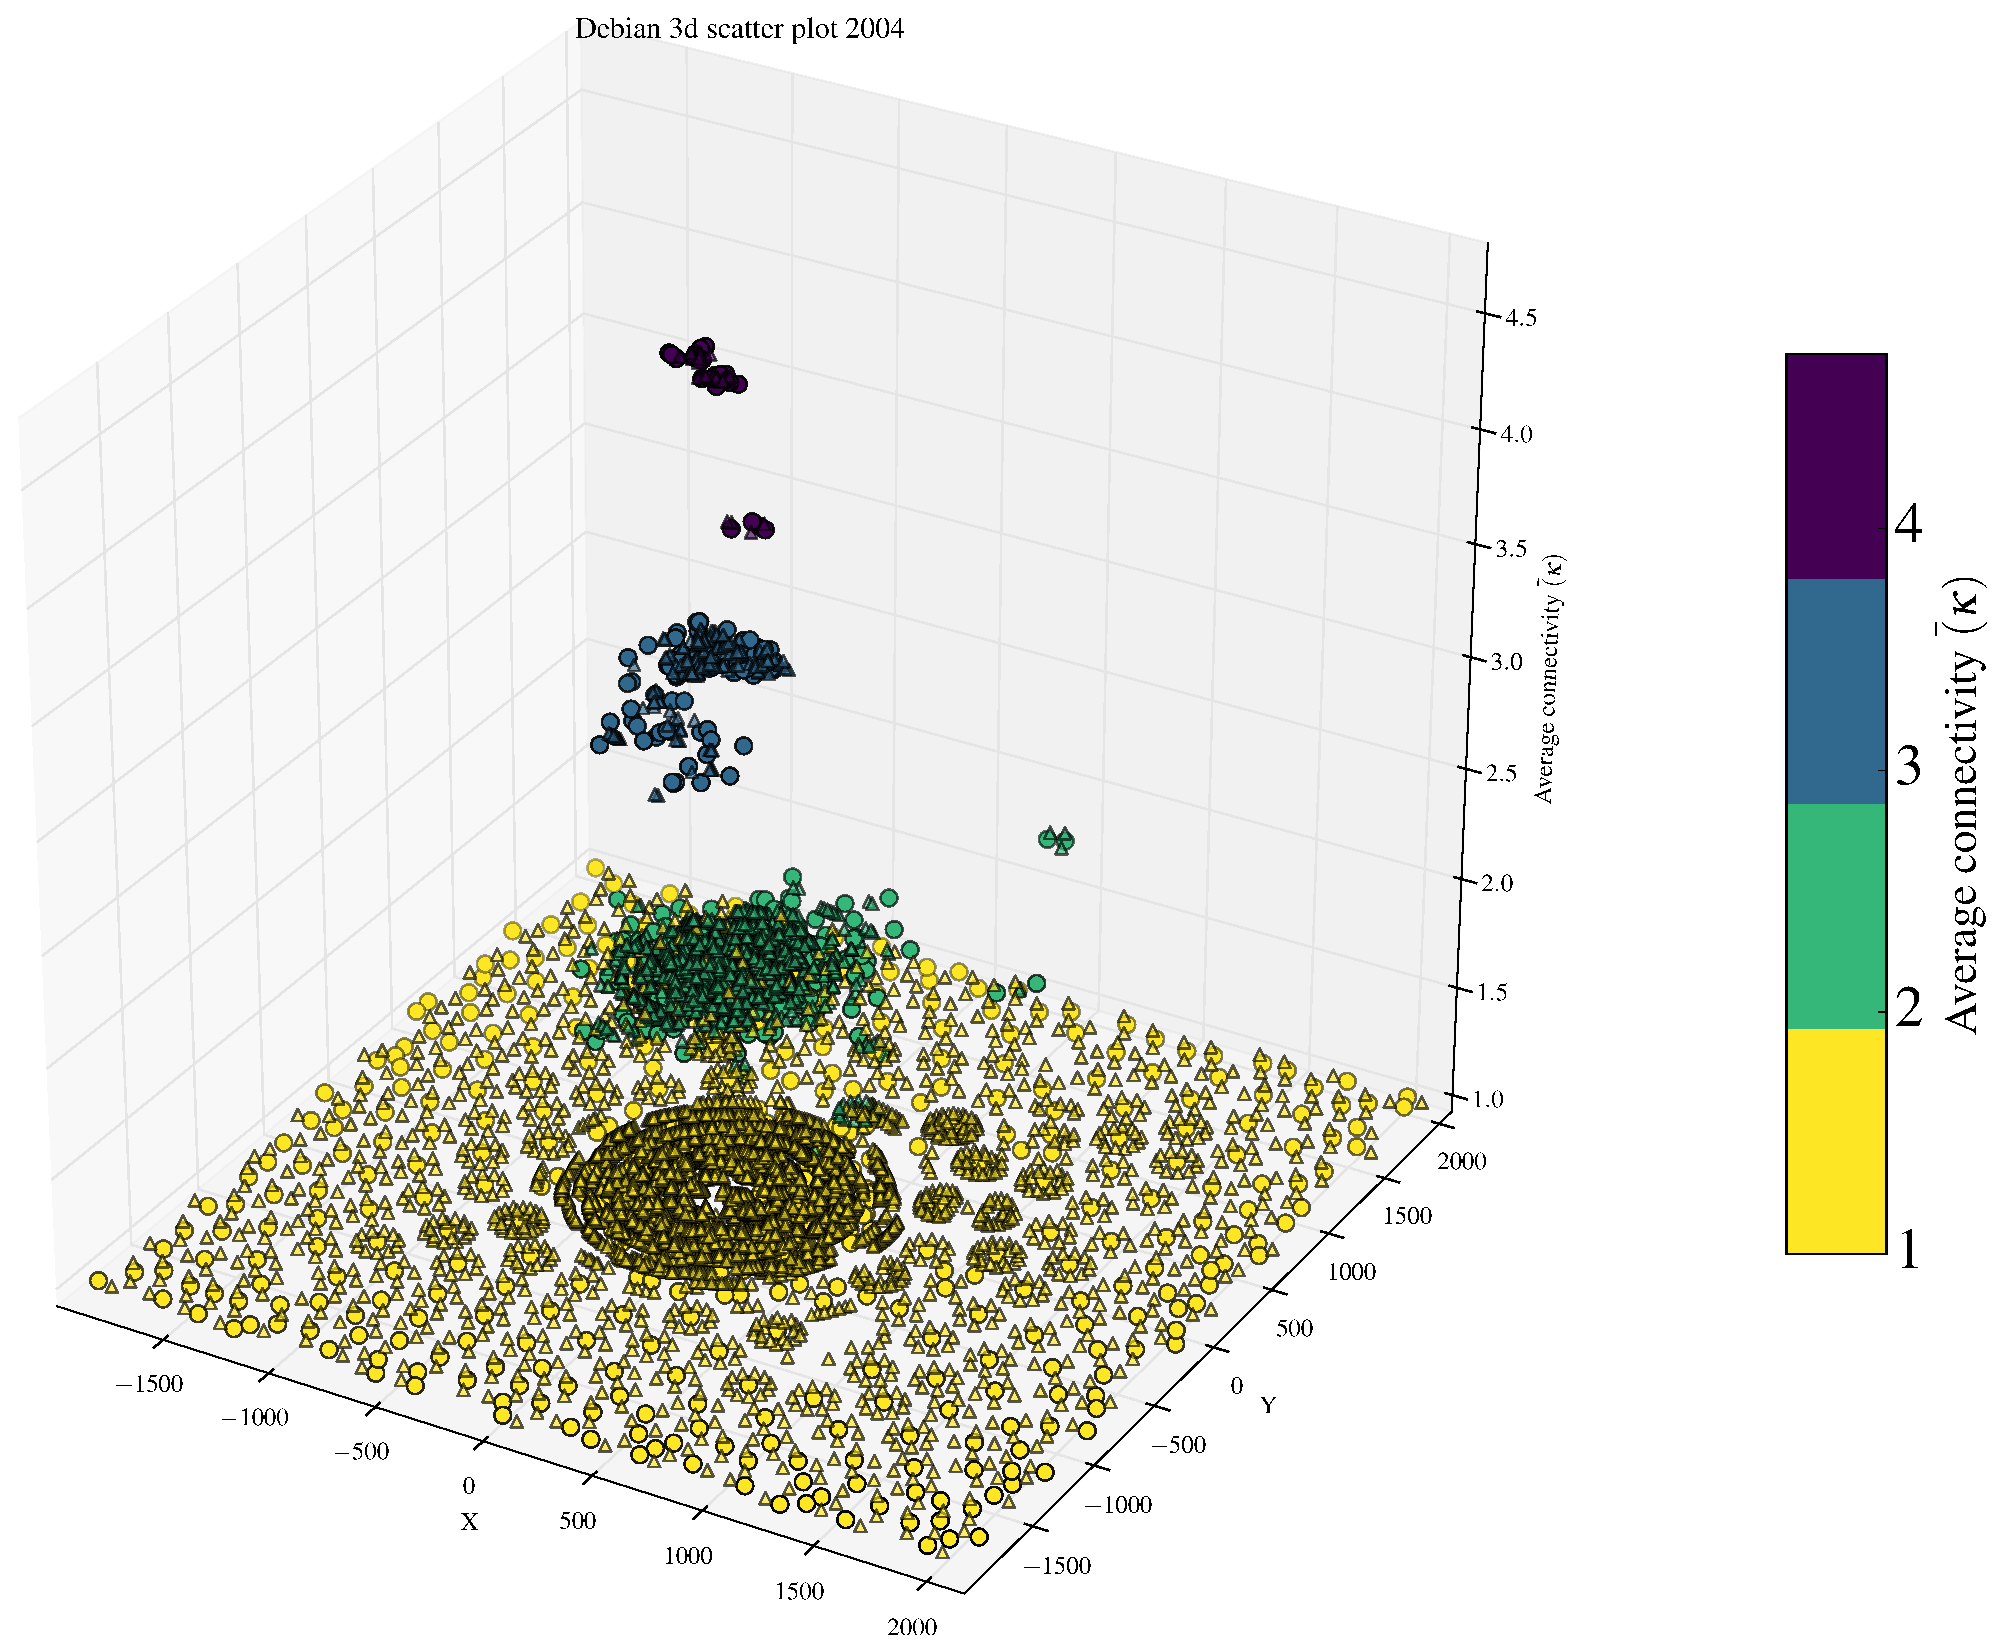
\includegraphics[scale=0.23]{figures/3d_scatter_debian_2004}
}
\hspace{.01in}
\subfloat[Null model Debian network 2004]{
\label{fig:s3d_null_debian_2004}
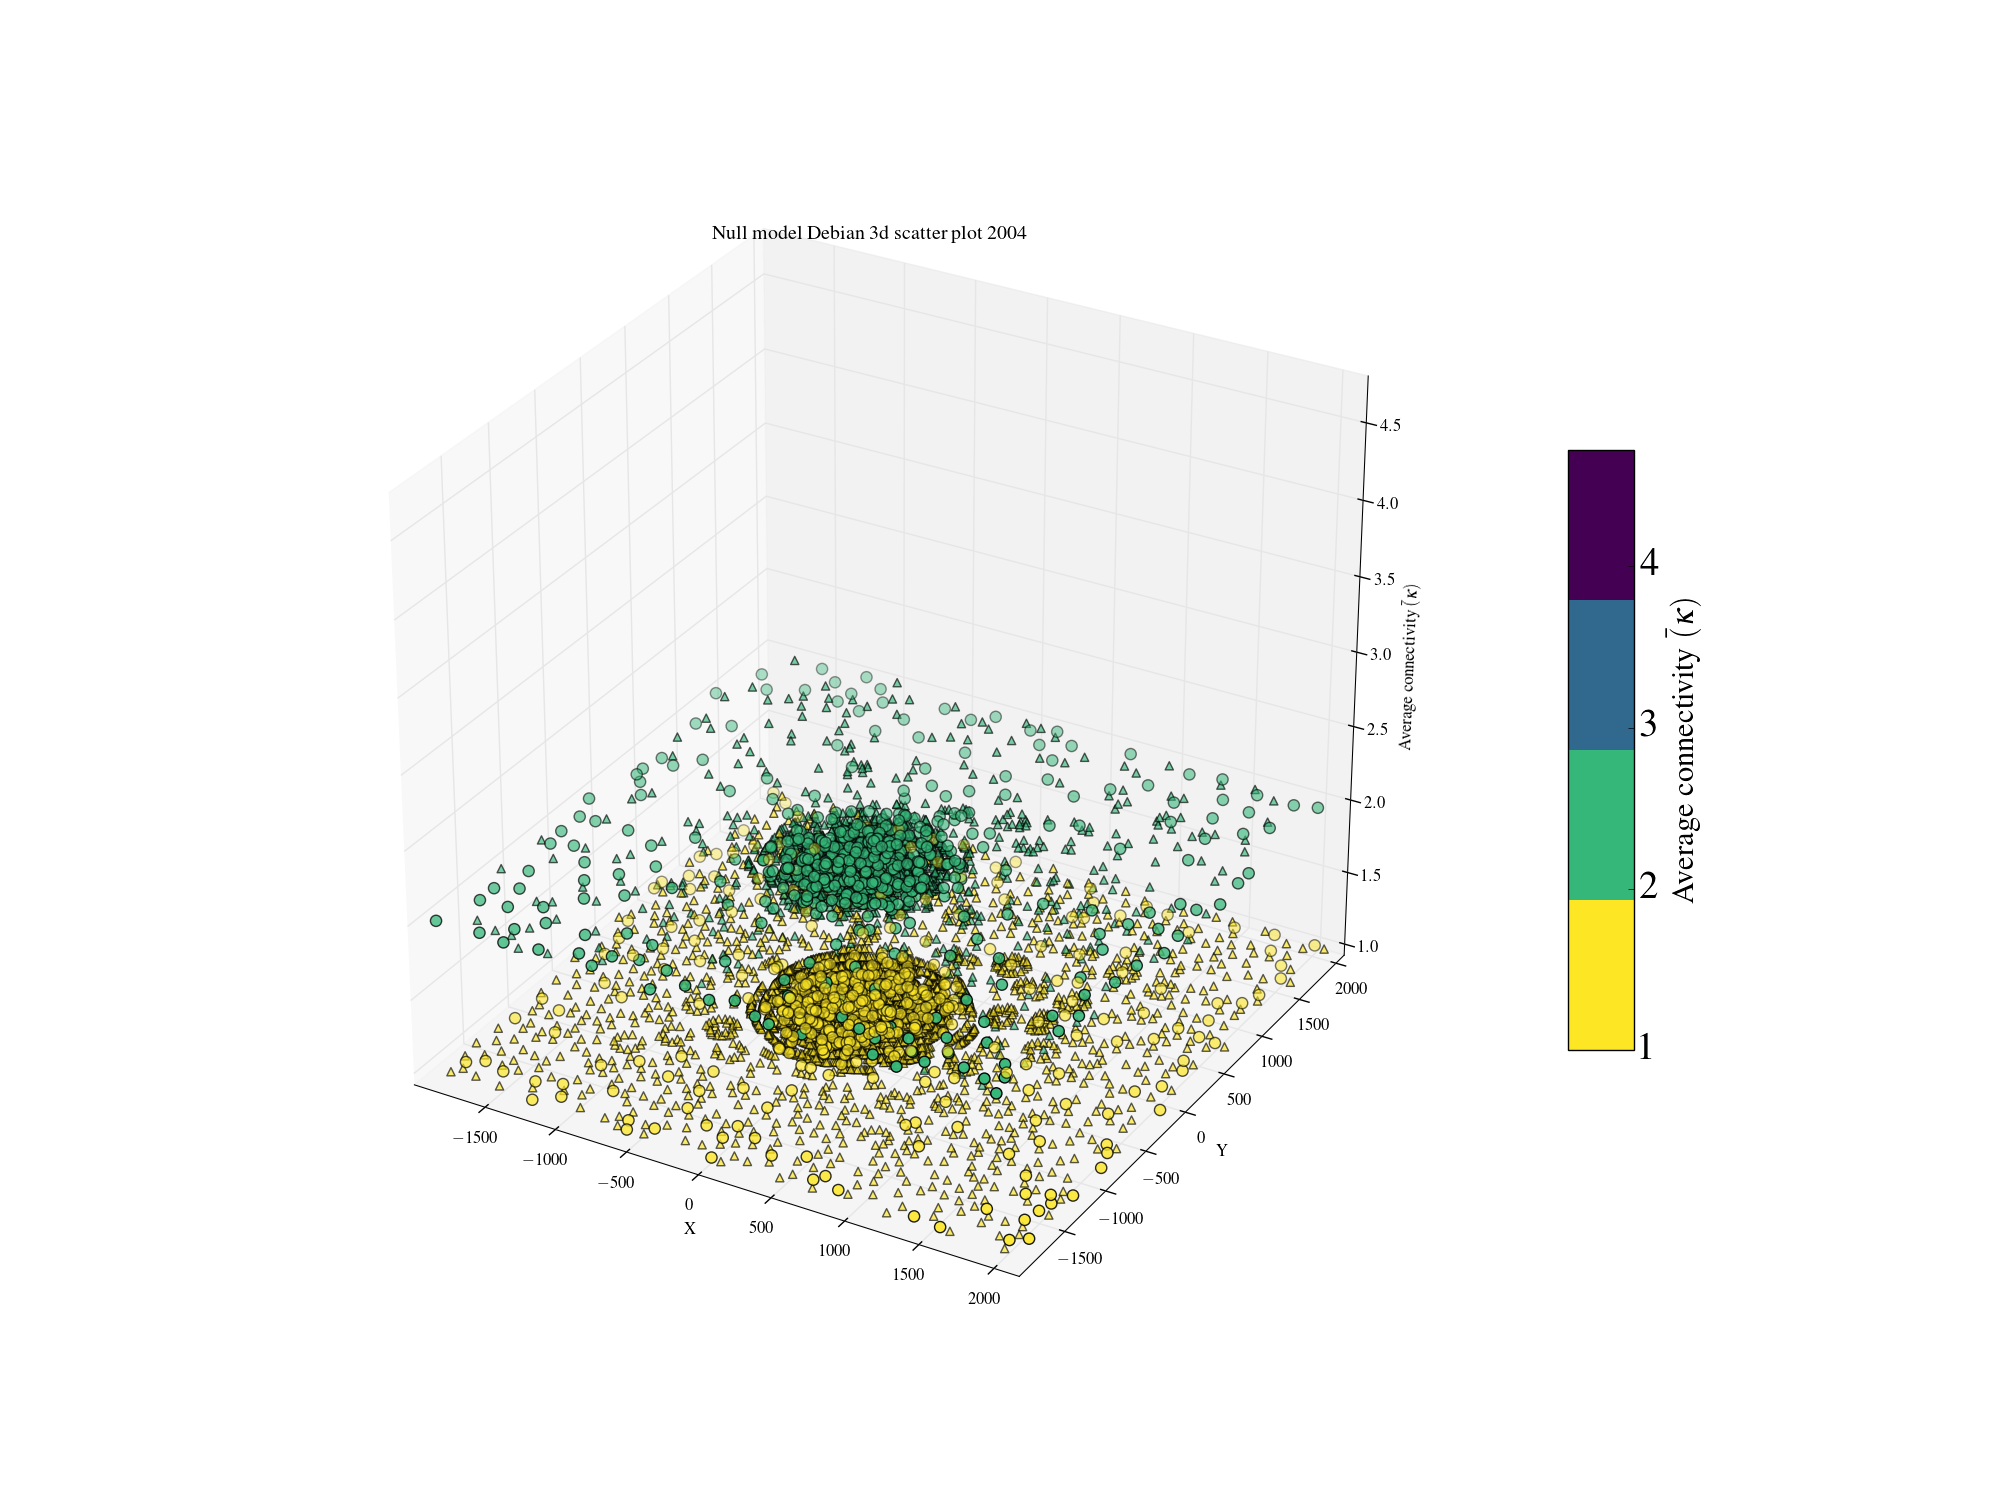
\includegraphics[scale=0.23]{figures/3d_scatter_debian_2004_null}
}

\subfloat[Actual Debian network 2011]{
\label{fig:s3d_actual_debian_2011}
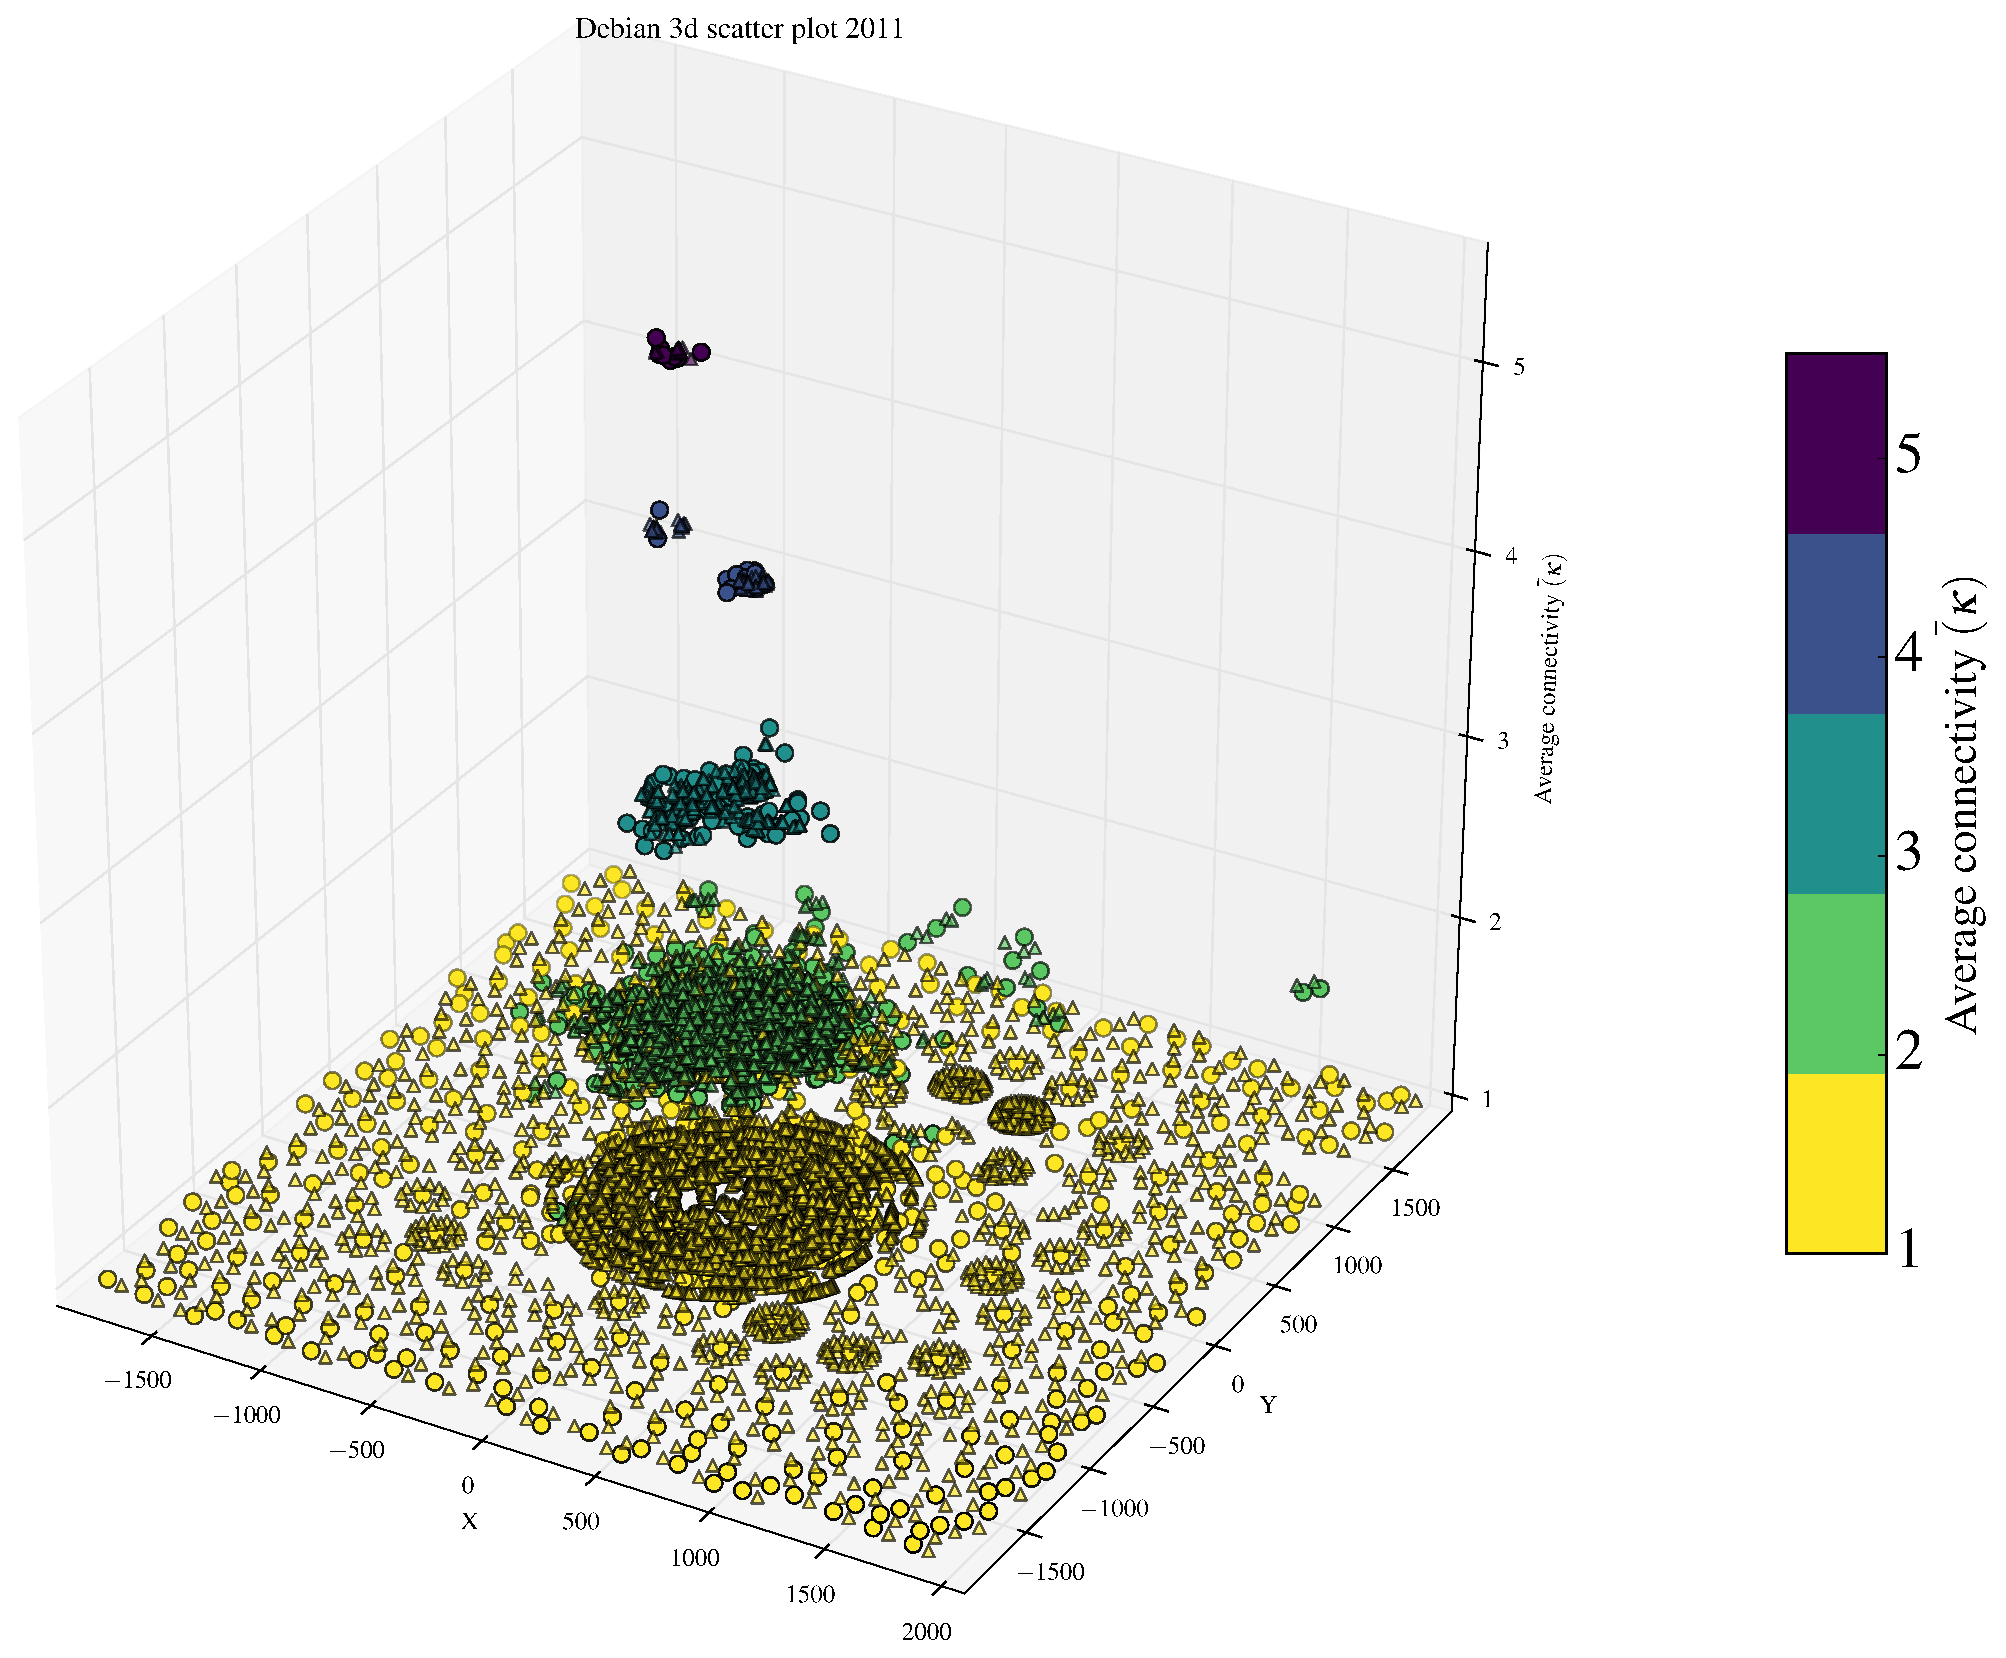
\includegraphics[scale=0.23]{figures/3d_scatter_debian_2011}
}
\hspace{.01in}
\subfloat[Null model Debian network 2011]{
\label{fig:s3d_null_debian_2011}
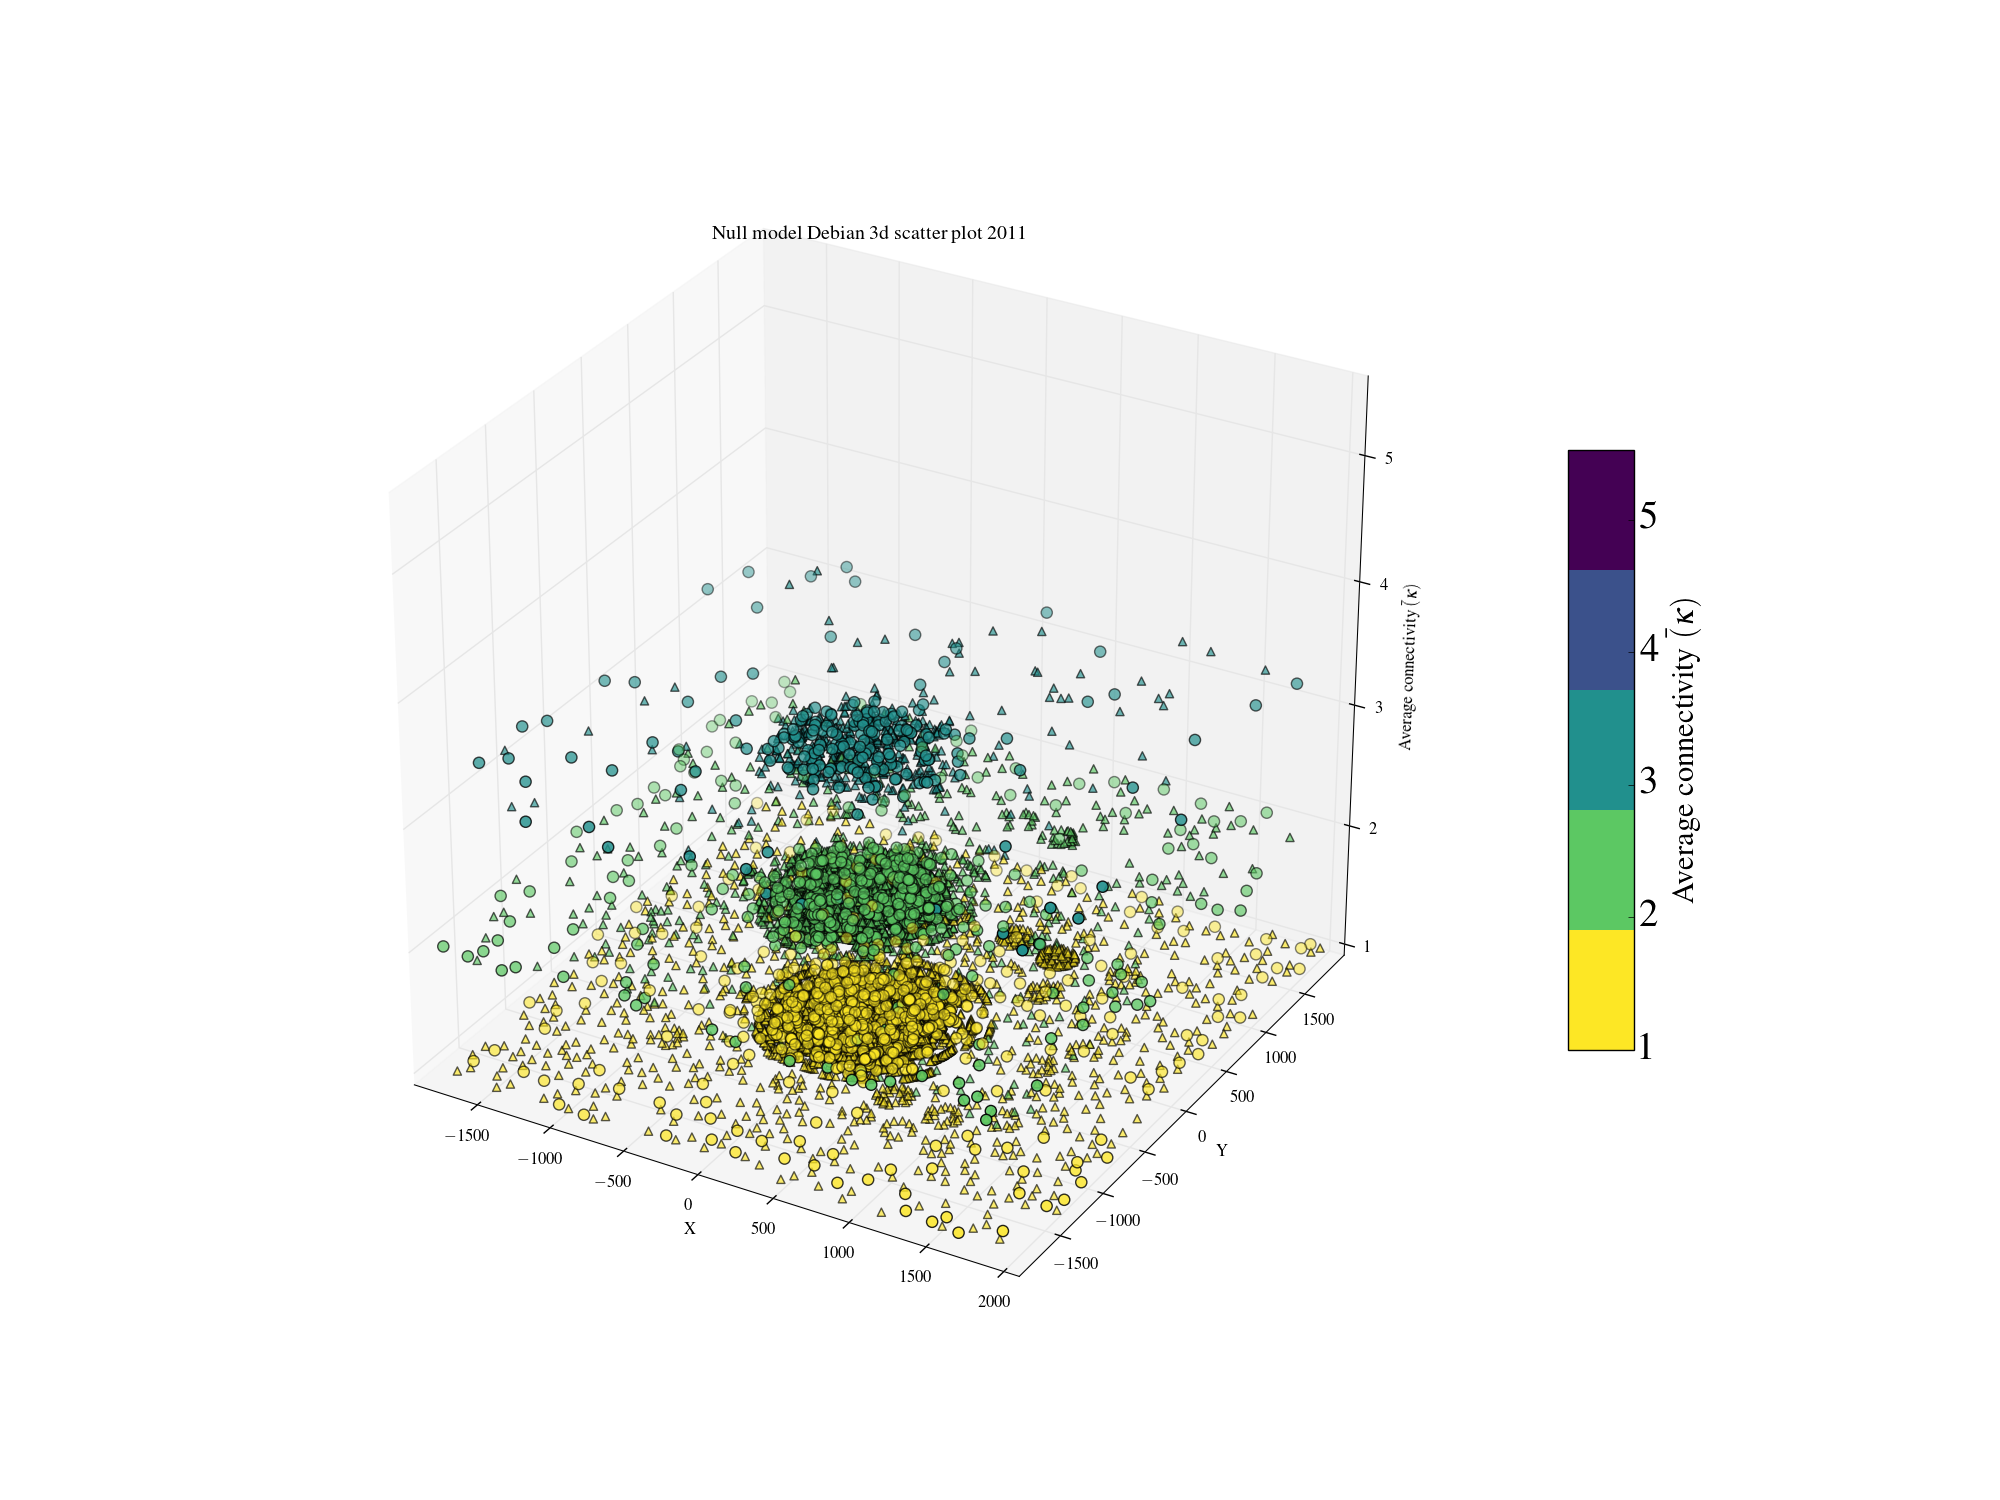
\includegraphics[scale=0.23]{figures/3d_scatter_debian_2011_null}
}

\caption[Debian average connectivity three-dimensional scatter plots.]{Debian average connectivity three-dimensional scatter plots for actual networks and their random null models counterparts. X and Y are the positions determined by the Kamada-Kawai layout algorithm. The vertical dimension is average connectivity. Each mark is a node of the network as two-mode networks they contain both programs (triangles) and developers (circles).}
\label{fig:debian-s3d}
\end{figure}
